\chapter{Experimentos e resultados}
\label{chap:Experimentos e resultados}
\lettrine{N}{este} capítulo presentaranse os experimentos realizados e os resultados obtidos.
Para iso, comezarase presentando unha vista xeral do proceso de experimentación, 
seguido dos propios experimentos realizados, para 
Finalmente analizar os resultados obtidos en conxunto e as conclusións que se poden extraer deles.

\section{Vista Xeral}
\label{sec:Vista Xeral}

definiciones generales?

O obxetivo do traballo é determinar se as redes implícitas son aptas para a tarefa de rexistro de retinas.
Aínda tomando o traballo de IDIR como punto de partida, a tarefa de rexistro de retinas é substancialmente diferente á de pulmóns, polo que non podemos asumir que os parámetros utilizados nese caso sexan os óptimos para este.

A principal comparación que estamos a realizar ao longo de todos os experimentos é sobre a función de activación utilizada (SIREN ou ReLU).
Debido ao gran espazo de búsqueda que implica probar todas as configuracións posibles, 
os experimentos iniciais cetraránse en fixar unha unha seria de parámetros con valores razonables para poder experimentar só con aqueles que podan ter un impacto máis significativo.

Ademais, debido ás diferencias entre as funcións de activación, cada unha require unha configuración diferente para obter os mellores resultados.
Por exemplo, SIREN tende a requerir de dun learning rate mais baixo que ReLU, presumiblemente debido a unha maior sensibilidade aos valores de inicialización e inesabilidade.
probar?

\section{Experimentos}
\label{sec:Experimentos}

\subsection{Experimentos iniciais}
\label{subsec:Experimentos iniciais}

Inicialmente tentaremos determinar uns valores aceptables para varios dos parámetros da rede para experimentar con aqueles que teñen un impacto máis significativo posteriormente.
Isto é relevante xa que moitos destes parámetros son dependentes uns de outros (por exemplo, a resolución utilizada inflúe no tamaño do batch size).

\subsubsection{Función de loss}
\label{subsubsec:Función de loss}

\paragraph{Planteamento}
\label{par:Planteamento}

A función de loss é un dos aspectos máis importantes á hora de entrenar unha rede neuronal.
As funcións de perda valoradas para este traballo xa forón explicadas en \ref{subsubsec:Termos de loss}.

Para determinar cal é a función de perda mais adecuada para a tarefa de rexistro de retinas, realizáronse experimentos comparando o rendemento de cada unha sobre unha mostra de imaxes dos datases de FIRE e RFMID.
Xa que a rede non é capaz de rexistrar con éxito a gran parte das imaxes, tomaráse a distancia media de todos os puntos como métrica de comparación.
Utilizouse un valor de batch size de 10000 puntos e un learning rate de 0.0001, ao longo de 1500 epochs con regularización de bending e hyper con valores de 50 e 0.25 respectivamente.

\paragraph{Resultados}
\label{par:Resultados}

Os resultados obtidos son os seguintes:

% \begin{table}[h]
%     \centering
%     \begin{tabular}{|l|c|c|}
%     \hline
%     Loss Function & FIRE Mean Distance & RFMID Mean Distance \\ \hline
%     ncc & 250.59 & 36.04 \\ \hline
%     mse & 392.94 & 9.50 \\ \hline
%     l1 & 404.83 & 5.42 \\ \hline
%     smoothl1 & 414.79 & 7.01 \\ \hline
%     \end{tabular}
%     \caption{Distancias medias según a función de perda. Valores máis baixos son mellores.}
%     \label{tab:mean_distances}
% \end{table}


\begin{table}[h]
    \centering
    \begin{tabular}{|l|cc|cc|}
    \hline
    \multirow{2}{*}{Loss Function} & \multicolumn{2}{c|}{FIRE Dataset} & \multicolumn{2}{c|}{RFMID Dataset} \\ \cline{2-5}
     & Relu & SIREN & Relu & SIREN \\ \hline
    huber & 399.86 & 397.45 & 7.13 & 57.31 \\ \hline
    l1 & 404.83 & 391.87 & 5.42 & 52.91 \\ \hline
    mse & 392.94 & 410.97 & 9.50 & 121.54 \\ \hline
    ncc & 250.59 & 281.03 & 36.04 & 79.84 \\ \hline
    smoothl1 & 414.79 & 387.71 & 7.01 & 60.74 \\ \hline
    ssim & 268.72 & 264.98 & 23.34 & 55.07 \\ \hline
    \end{tabular}
    \caption{Distancias medias segundo función de perda, tipo de rede e datasets (FIRE vs. RFMID)}
    \label{tab:mean_distances}
\end{table}

\begin{figure}[h]
    \centering
    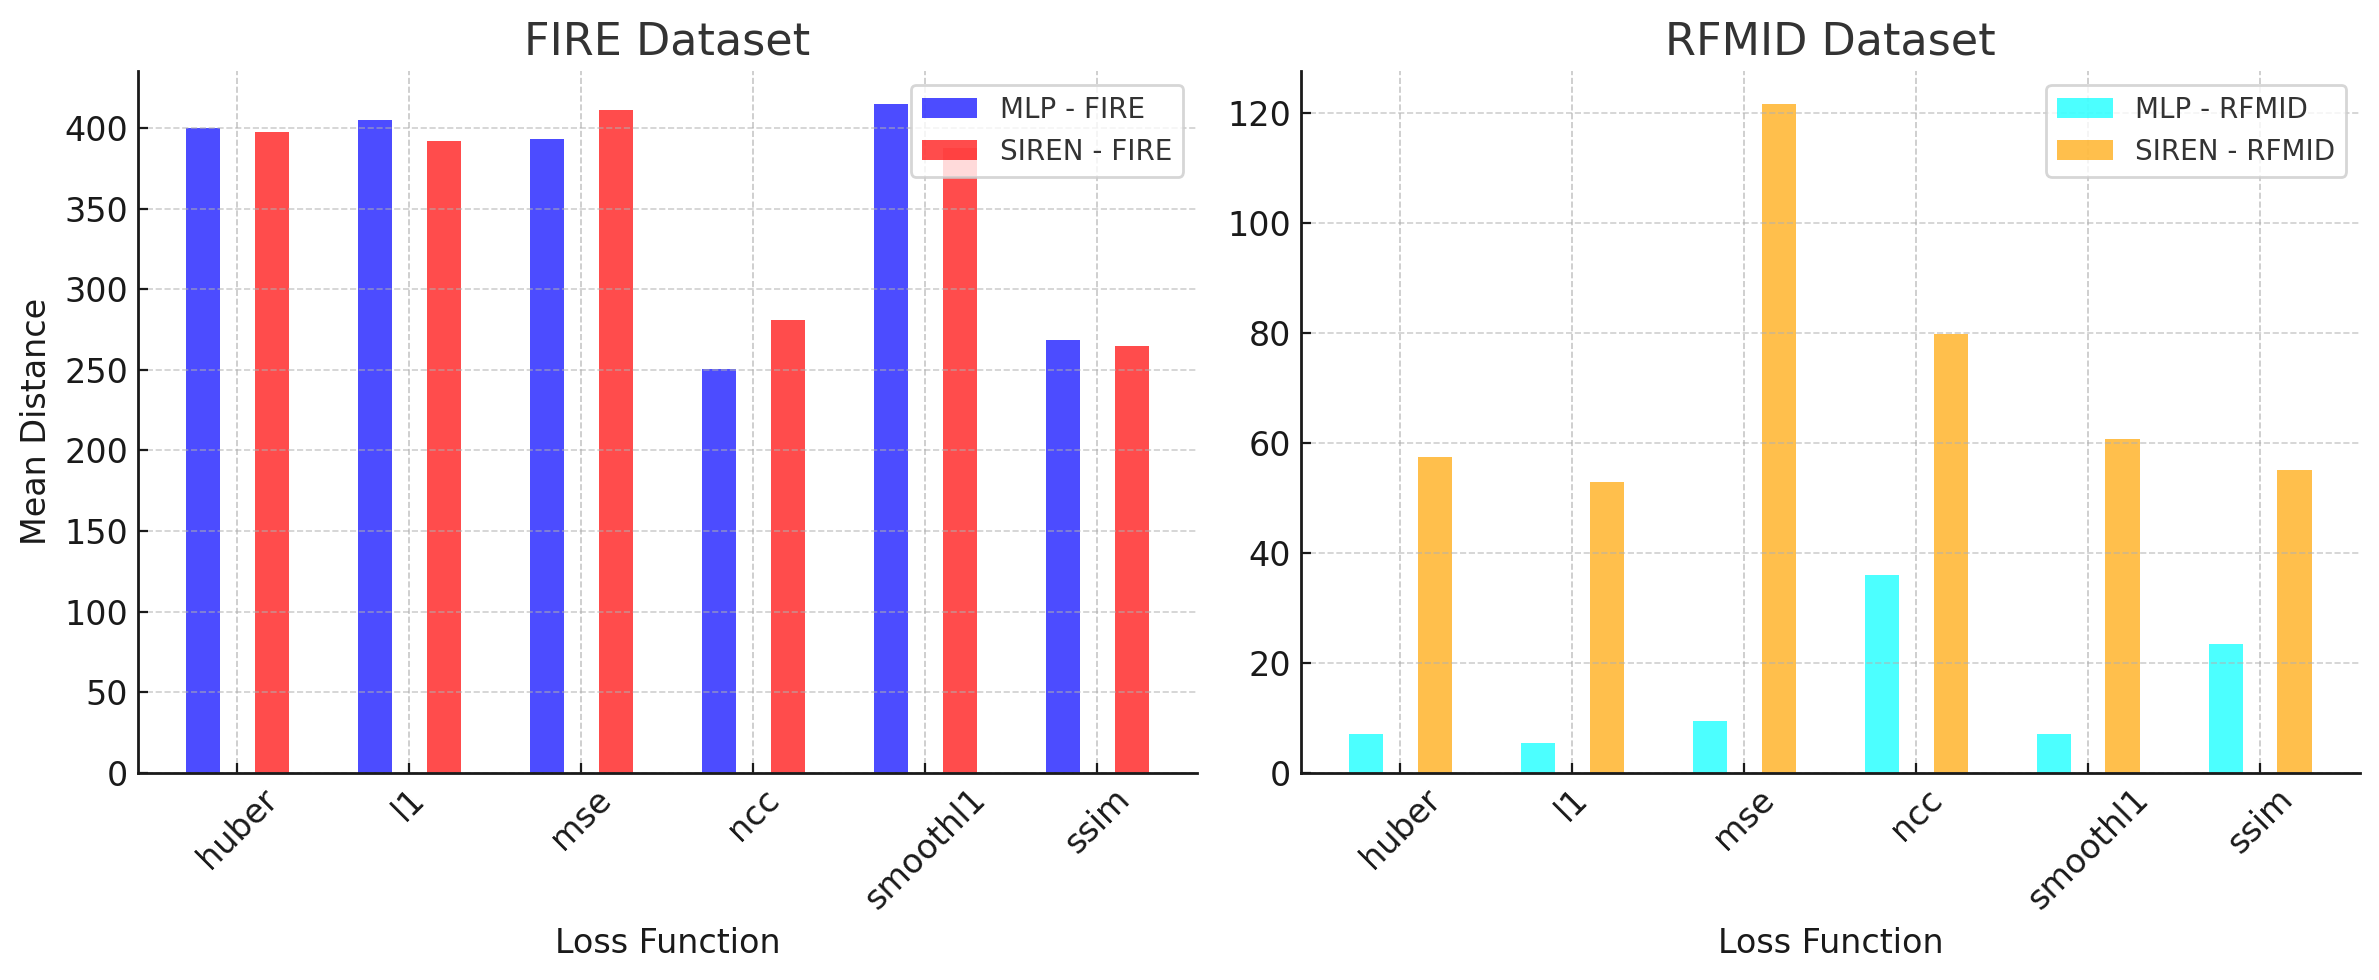
\includegraphics[width=0.75\textwidth]{imaxes/losstype.png}
    \caption{Comparación de diferentes funcións de perda sobre imaxes de FIRE e RFMID}
    \label{fig:loss_functions_comparison}
\end{figure}
    


\paragraph{Discusión}
\label{par:Discusión}

Obsérvase como as métricas que teñen en conta a estructura da imaxe (NCC, Ssim) tenden a dar mellores resultados que aquelas que non o fan (MSE, Huber, Smooth L1) co dataset de FIRE, mentres que con RFMID ocurre ó contrario.
Isto pode deberse a que as imaxes reais de retina teñen unha maior variabilidade na iluminación e contraste, polo que as métricas que non teñen en conta a estructura da imaxe serán menos robustas a estas diferenzas.
No caso de RFMID, ao ser imaxes sintéticas, a variabilidade na iluminación e contraste é nula, o que explica os mellores resultados das métricas que non teñen en conta a estructura da imaxe.

NCC é mais robusta a combios uniformes na intensidade global, mentres que SSIM é mais robusta a cambios locais a custo dun maior custo computacional e maior sensibilidade a ruido e o tamaño das seccións.
SSIM puede que no tenga mucho sentido ya que para calcular el loss se comparan solo los puntos sampleados de la imagen, que no tienen una estructura definida o que aporte mucha información.
Reconstruir la imagen en cada iteracion era computacionalmente muy costoso.
\paragraph{Conclusións}
\label{par:Conclusións}

\paragraph{Conclusións}
\label{par:Conclusións}

En base aos resultados obtidos, pódense extraer varias conclusións relevantes:

1. Para o dataset FIRE, que contén imaxes reais de retina con variabilidade en iluminación e contraste, as funcións de perda baseadas en características estruturais como NCC e SSIM proporcionan resultados significativamente mellores. En particular, NCC mostra o menor erro medio (250.59 para Relu e 281.03 para SIREN).
2. Para o dataset RFMID, que contén imaxes con tan só variación xeométrica, as funcións de perda baseadas en píxeles como L1 e Smooth L1 ofrecen mellores resultados. Concretamente, L1 presenta o menor erro medio para Relu (5.42) e resultados competitivos para SIREN (52.91).
3. Obsérvase unha diferenza sistemática entre os modelos Relu e SIREN, sendo os primeiros máis efectivos para o dataset RFMID, mentres que ambos mostran rendementos comparables para FIRE. Isto débese a que Relu tende a producir funcións predominantemente lineares, o que se adapta mellor ás transformacións realizadas no dataset RFMID.
4. SSIM, a pesar de ser teoricamente robusta a cambios locais, non mostra unha vantaxe significativa sobre NCC.

Considerando estes resultados, empregarase principalmente NCC como función de perda estándar para o dataset FIRE e RFMID.

\subsubsection{Resolución da imaxe}
\label{subsubsec:Resolución da imaxe}

\paragraph{Planteamento}
\label{par:Planteamento}

A resolución da imaxe é un aspecto clave xa que inflúe de forma directa no resto de parámetros da rede.
Por exemplo, un batch size de 1000 puntos nunha imaxe de 256x256 é unha densidade de puntos moito maior que nunha imaxe de 512x512.

Ademais, a resolución da imaxe tamén inflúe na capacidade da rede para aprender as transformacións, xa que a información que recibe é mais detallada. 
Isto pode ser beneficioso se estos detalles conteñen información relevante para a tarefa de rexistro, pero tamén podería ser perxudicial se conteñen unha gran parte de ruido.

O tamaño das imaxes tamén é unha das principais diferencias entre as imaxes de retina e as de pulmóns utilizadas orixinalmente por IDIR, tendo estas últimas de 512x512 e as primeiras de ata 2160x2160.

Para determinar cal é a resolución mais adecuada, realizáronse experimentos comparando o rendemento de cada unha sobre unha mostra de imaxes dos datases de FIRE e RFMID.
Debido a que a rede non é capaz de rexistrar con éxito a gran parte das imaxes, tomaráse a distancia media de todos os puntos como métrica de comparación.

\paragraph{Resultados}
\label{par:Resultados}

\begin{table}[h]
    \centering
    \begin{minipage}[t]{0.45\linewidth}
        \centering
        \begin{tabular}{|c|c|}
        \hline
        Resolution & Mean Distance \\ \hline
        250 & 251.29 \\ \hline
        750 & 250.62 \\ \hline
        1250 & 250.59 \\ \hline
        1708 & 249.72 \\ \hline
        \end{tabular}
        \caption{Mean Distances for Relu (FIRE)}
        \label{tab:mlp_mean_distances_fire}
    \end{minipage}
    \hfill
    \begin{minipage}[t]{0.45\linewidth}
        \centering
        \begin{tabular}{|c|c|}
        \hline
        Resolution & Mean Distance \\ \hline
        250 & 263.85 \\ \hline
        750 & 263.19 \\ \hline
        1250 & 258.56 \\ \hline
        1708 & 258.06 \\ \hline
        \end{tabular}
        \caption{Mean Distances for SIREN (FIRE)}
        \label{tab:siren_mean_distances_fire}
    \end{minipage}
\end{table}

\begin{table}[h]
    \centering
    \begin{minipage}[t]{0.45\linewidth}
        \centering
        \begin{tabular}{|c|c|}
        \hline
        Resolution & Mean Distance \\ \hline
        250 & 36.18 \\ \hline
        750 & 36.01 \\ \hline
        1250 & 35.03 \\ \hline
        1708 & 35.04 \\ \hline
        \end{tabular}
        \caption{Mean Distances for MLP (RFMID)}
        \label{tab:mlp_mean_distances_rfmid}
    \end{minipage}
    \hfill
    \begin{minipage}[t]{0.45\linewidth}
        \centering
        \begin{tabular}{|c|c|}
        \hline
        Resolution & Mean Distance \\ \hline
        250 & 73.42 \\ \hline
        750 & 77.55 \\ \hline
        1250 & 67.33 \\ \hline
        1708 & 67.31 \\ \hline
        \end{tabular}
        \caption{Mean Distances for SIREN (RFMID)}
        \label{tab:siren_mean_distances_rfmid}
    \end{minipage}
\end{table}

\paragraph{Discusión}
\label{par:Discusión}

Pódese observar como unha maior resolución tende a dar lixeiramente mellores resultados, pero a un custo computacional maior.
Isto pode deberse mais á precisión ca que se fai a evaluación mais que a unha mellor capacidade da rede para aprender as transformacións.


\paragraph{Conclusións}
\label{par:Conclusións}

Baseándonos nos resultados obtidos, podemos concluír que:

1. Resolucións inferiores a 512×512 non capturan suficientes detalles das estruturas vasculares retinianas para realizar un rexistro preciso, especialmente en imaxes reais do dataset FIRE.

2. Aumentar a resolución por encima de 1250x1250 non só non aporta beneficios significativos, senón que pode prexudicar o rendemento debido ao incremento na complexidade do modelo e á posible introdución de ruído nos detalles máis finos.

3. O comportamento respecto á resolución é consistente para ambos tipos de modelos (Relu e SIREN) e para ambos datasets (FIRE e RFMID), o que suxire que estas conclusións son xeneralizables para diferentes situacións de rexistro de imaxes retinianas.

Para os experimentos subseguintes, adoptarase unha resolución estándar de 1000x1000 píxeles, que demostrou proporcionar o mellor rendemento global para a tarefa de rexistro de retinas.

Podería ser interesante determinar cal é o punto de inflexión onde o aumento da resolución non compensa o aumento do rendemento.

\subsubsection{Regularización}
\label{subsubsec:Regularización}

\paragraph{Planteamento}
\label{par:Planteamento}

O proceso de regularización axuda a rede a evitar o sobreaxuste, modificando o termo de loss para penalizar as transformacións pouco realistas.
As técnicas de regularización valoradas para este traballo xa forón explicadas en \ref{subsubsec:Termos de regularización}.

\begin{itemize}
    \item Jacobian regularizer
    \item Hyperelastic regularizer
    \item Bending energy penalty
\end{itemize}

Se os termos de regularización son demasiado grandes, a rede fará transformacións moi pequenas para evitar ser penalizada, o que resulta nunha transformación insuficiente.
Por outro lado, se os termos son demasiado pequenos, a rede fará transformacións moi grandes, o que resulta nunha transformación irrealista e sobreaxustada.
A cantidade óptima de regularización depende da parexa concreta de imaxes a alinear, polo que intentaremos determinar cal é a mellor para unha mostra de imaxes ...

\paragraph{Resultados}
\label{par:Resultados}

\begin{figure}[ht]
    \centering
    \begin{subfigure}[b]{0.45\textwidth}
        \centering
        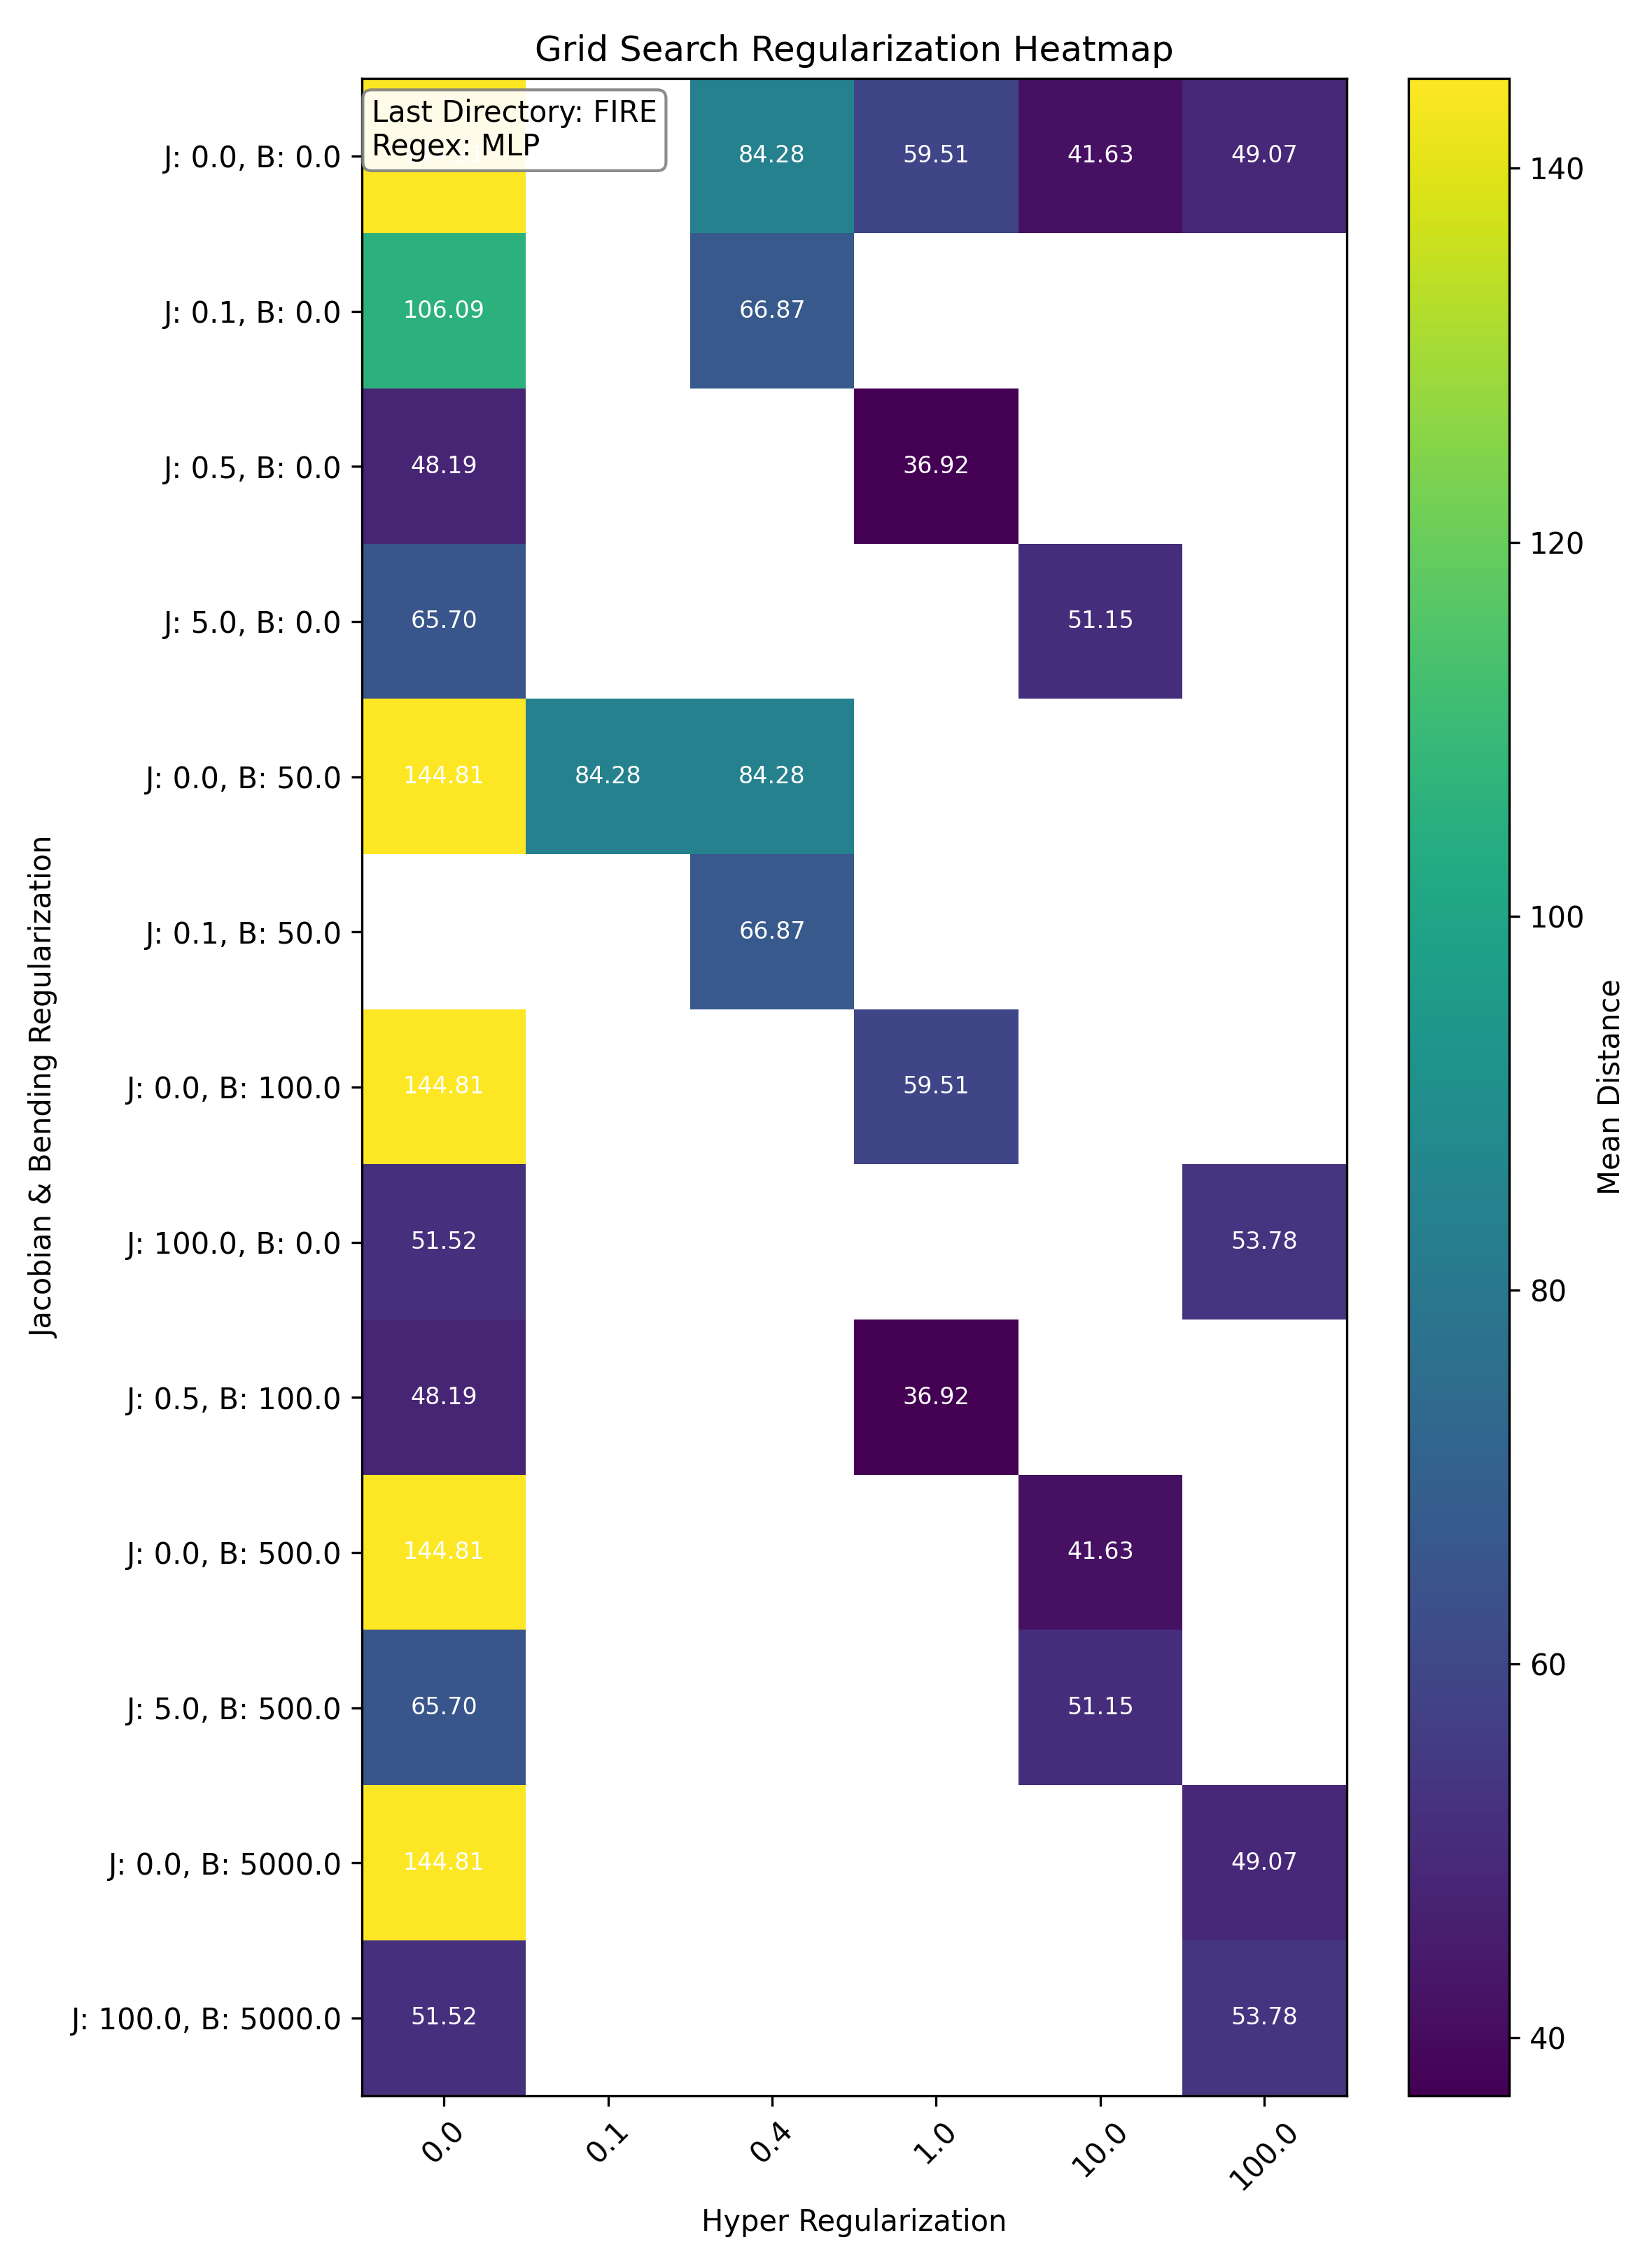
\includegraphics[width=\textwidth]{imaxes/grid_search_single_heatmap_FIRE_MLP.png}
        \caption{FIRE - Relu}
        \label{fig:gs_single_FIRE_MLP}
    \end{subfigure}\hfill
    \begin{subfigure}[b]{0.45\textwidth}
        \centering
        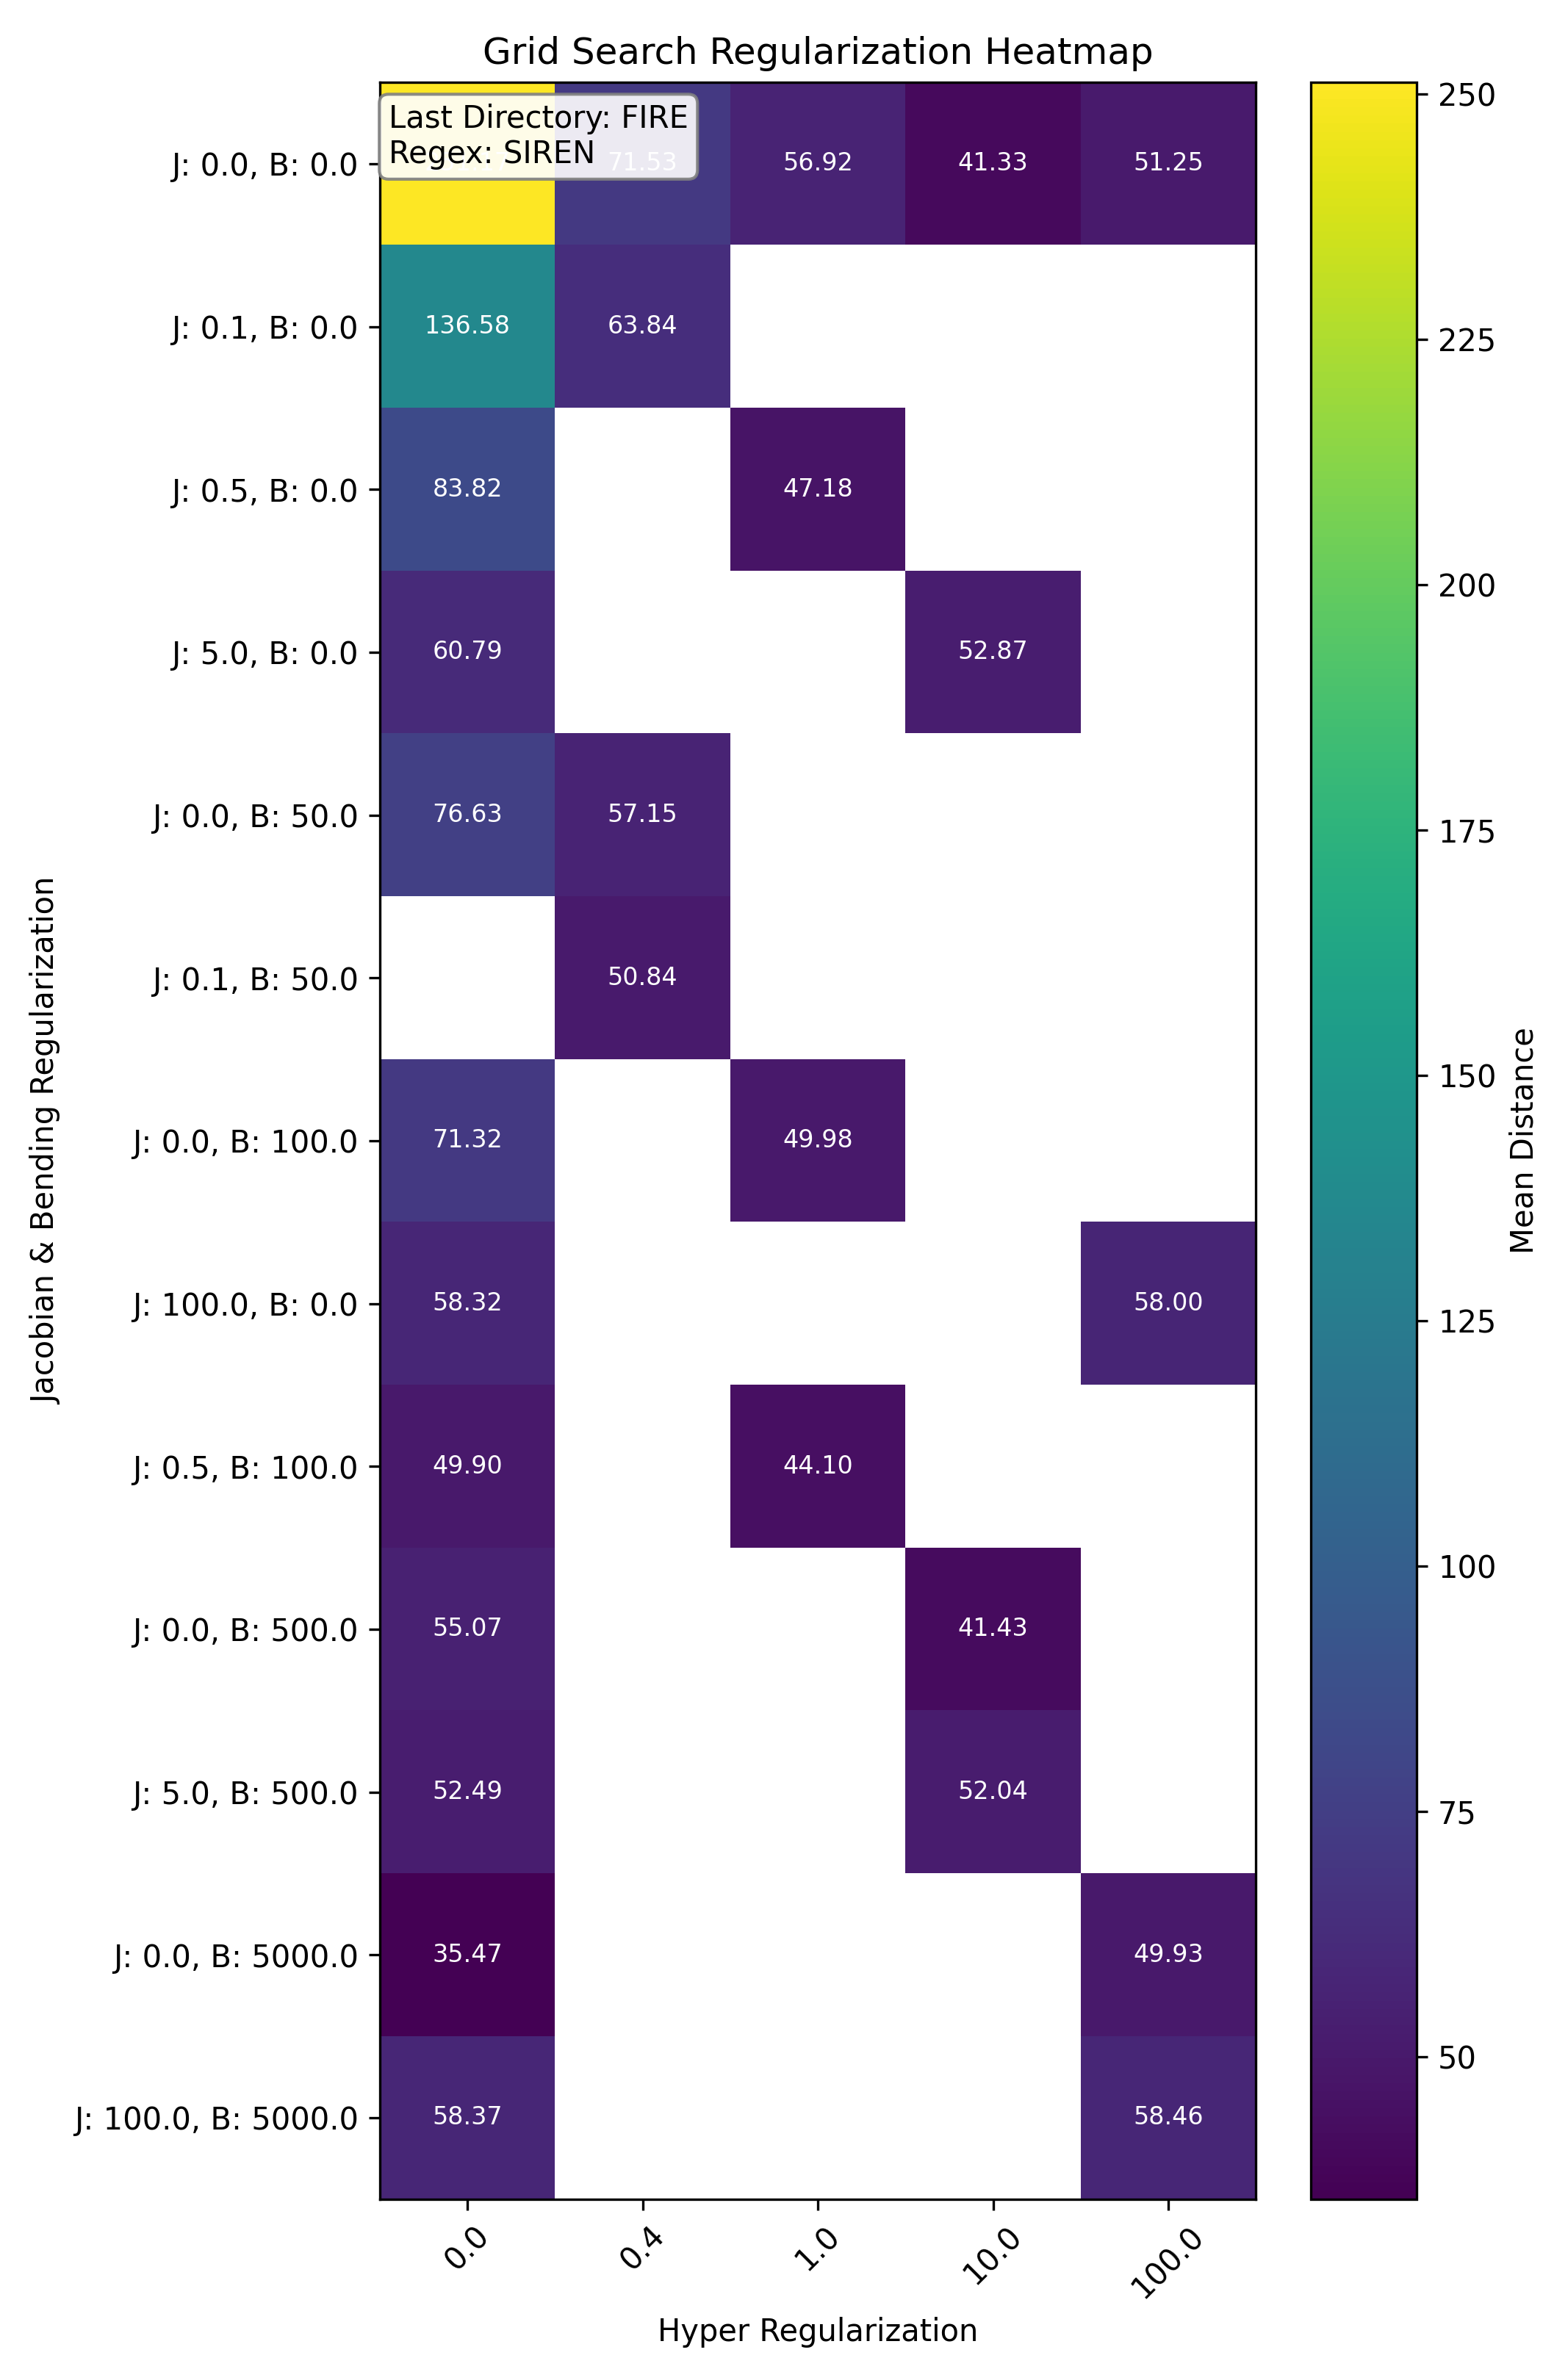
\includegraphics[width=\textwidth]{imaxes/grid_search_single_heatmap_FIRE_SIREN.png}
        \caption{FIRE - SIREN}
        \label{fig:gs_single_FIRE_SIREN}
    \end{subfigure}
    
    \vskip\baselineskip
    
    \begin{subfigure}[b]{0.45\textwidth}
        \centering
        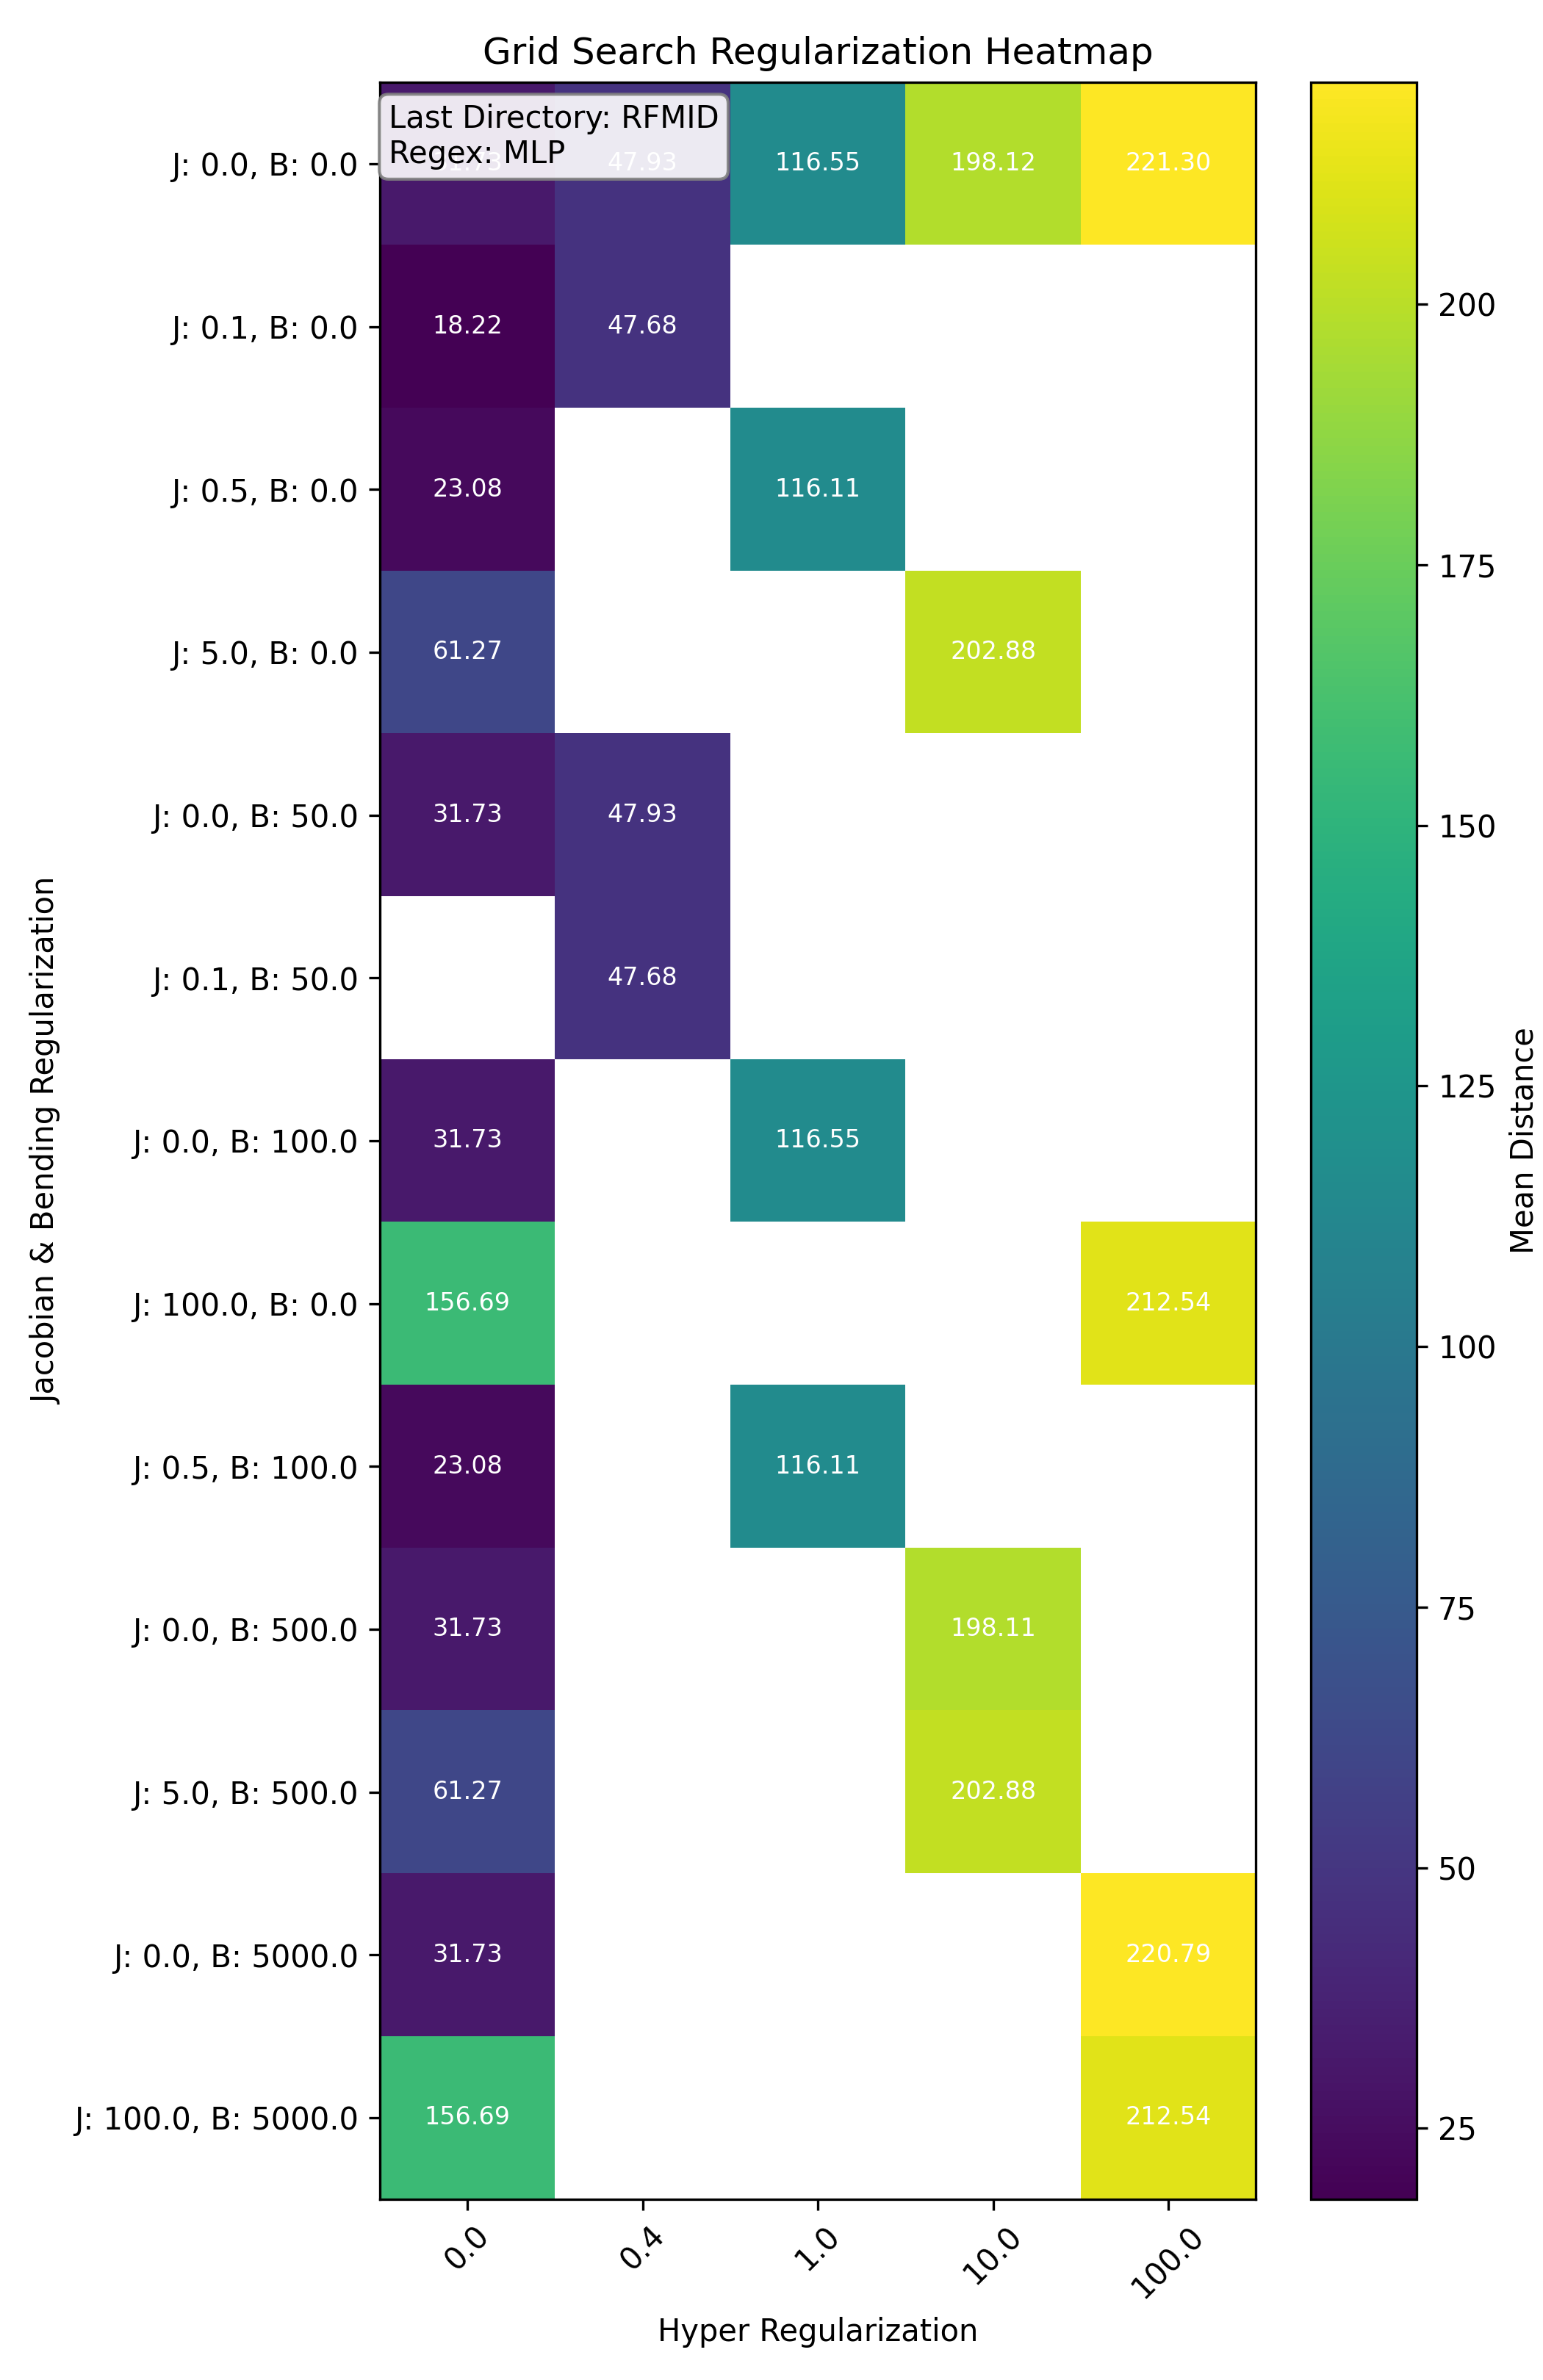
\includegraphics[width=\textwidth]{imaxes/grid_search_single_heatmap_RFMID_MLP.png}
        \caption{RFMID - Relu}
        \label{fig:gs_single_RFMID_MLP}
    \end{subfigure}\hfill
    \begin{subfigure}[b]{0.45\textwidth}
        \centering
        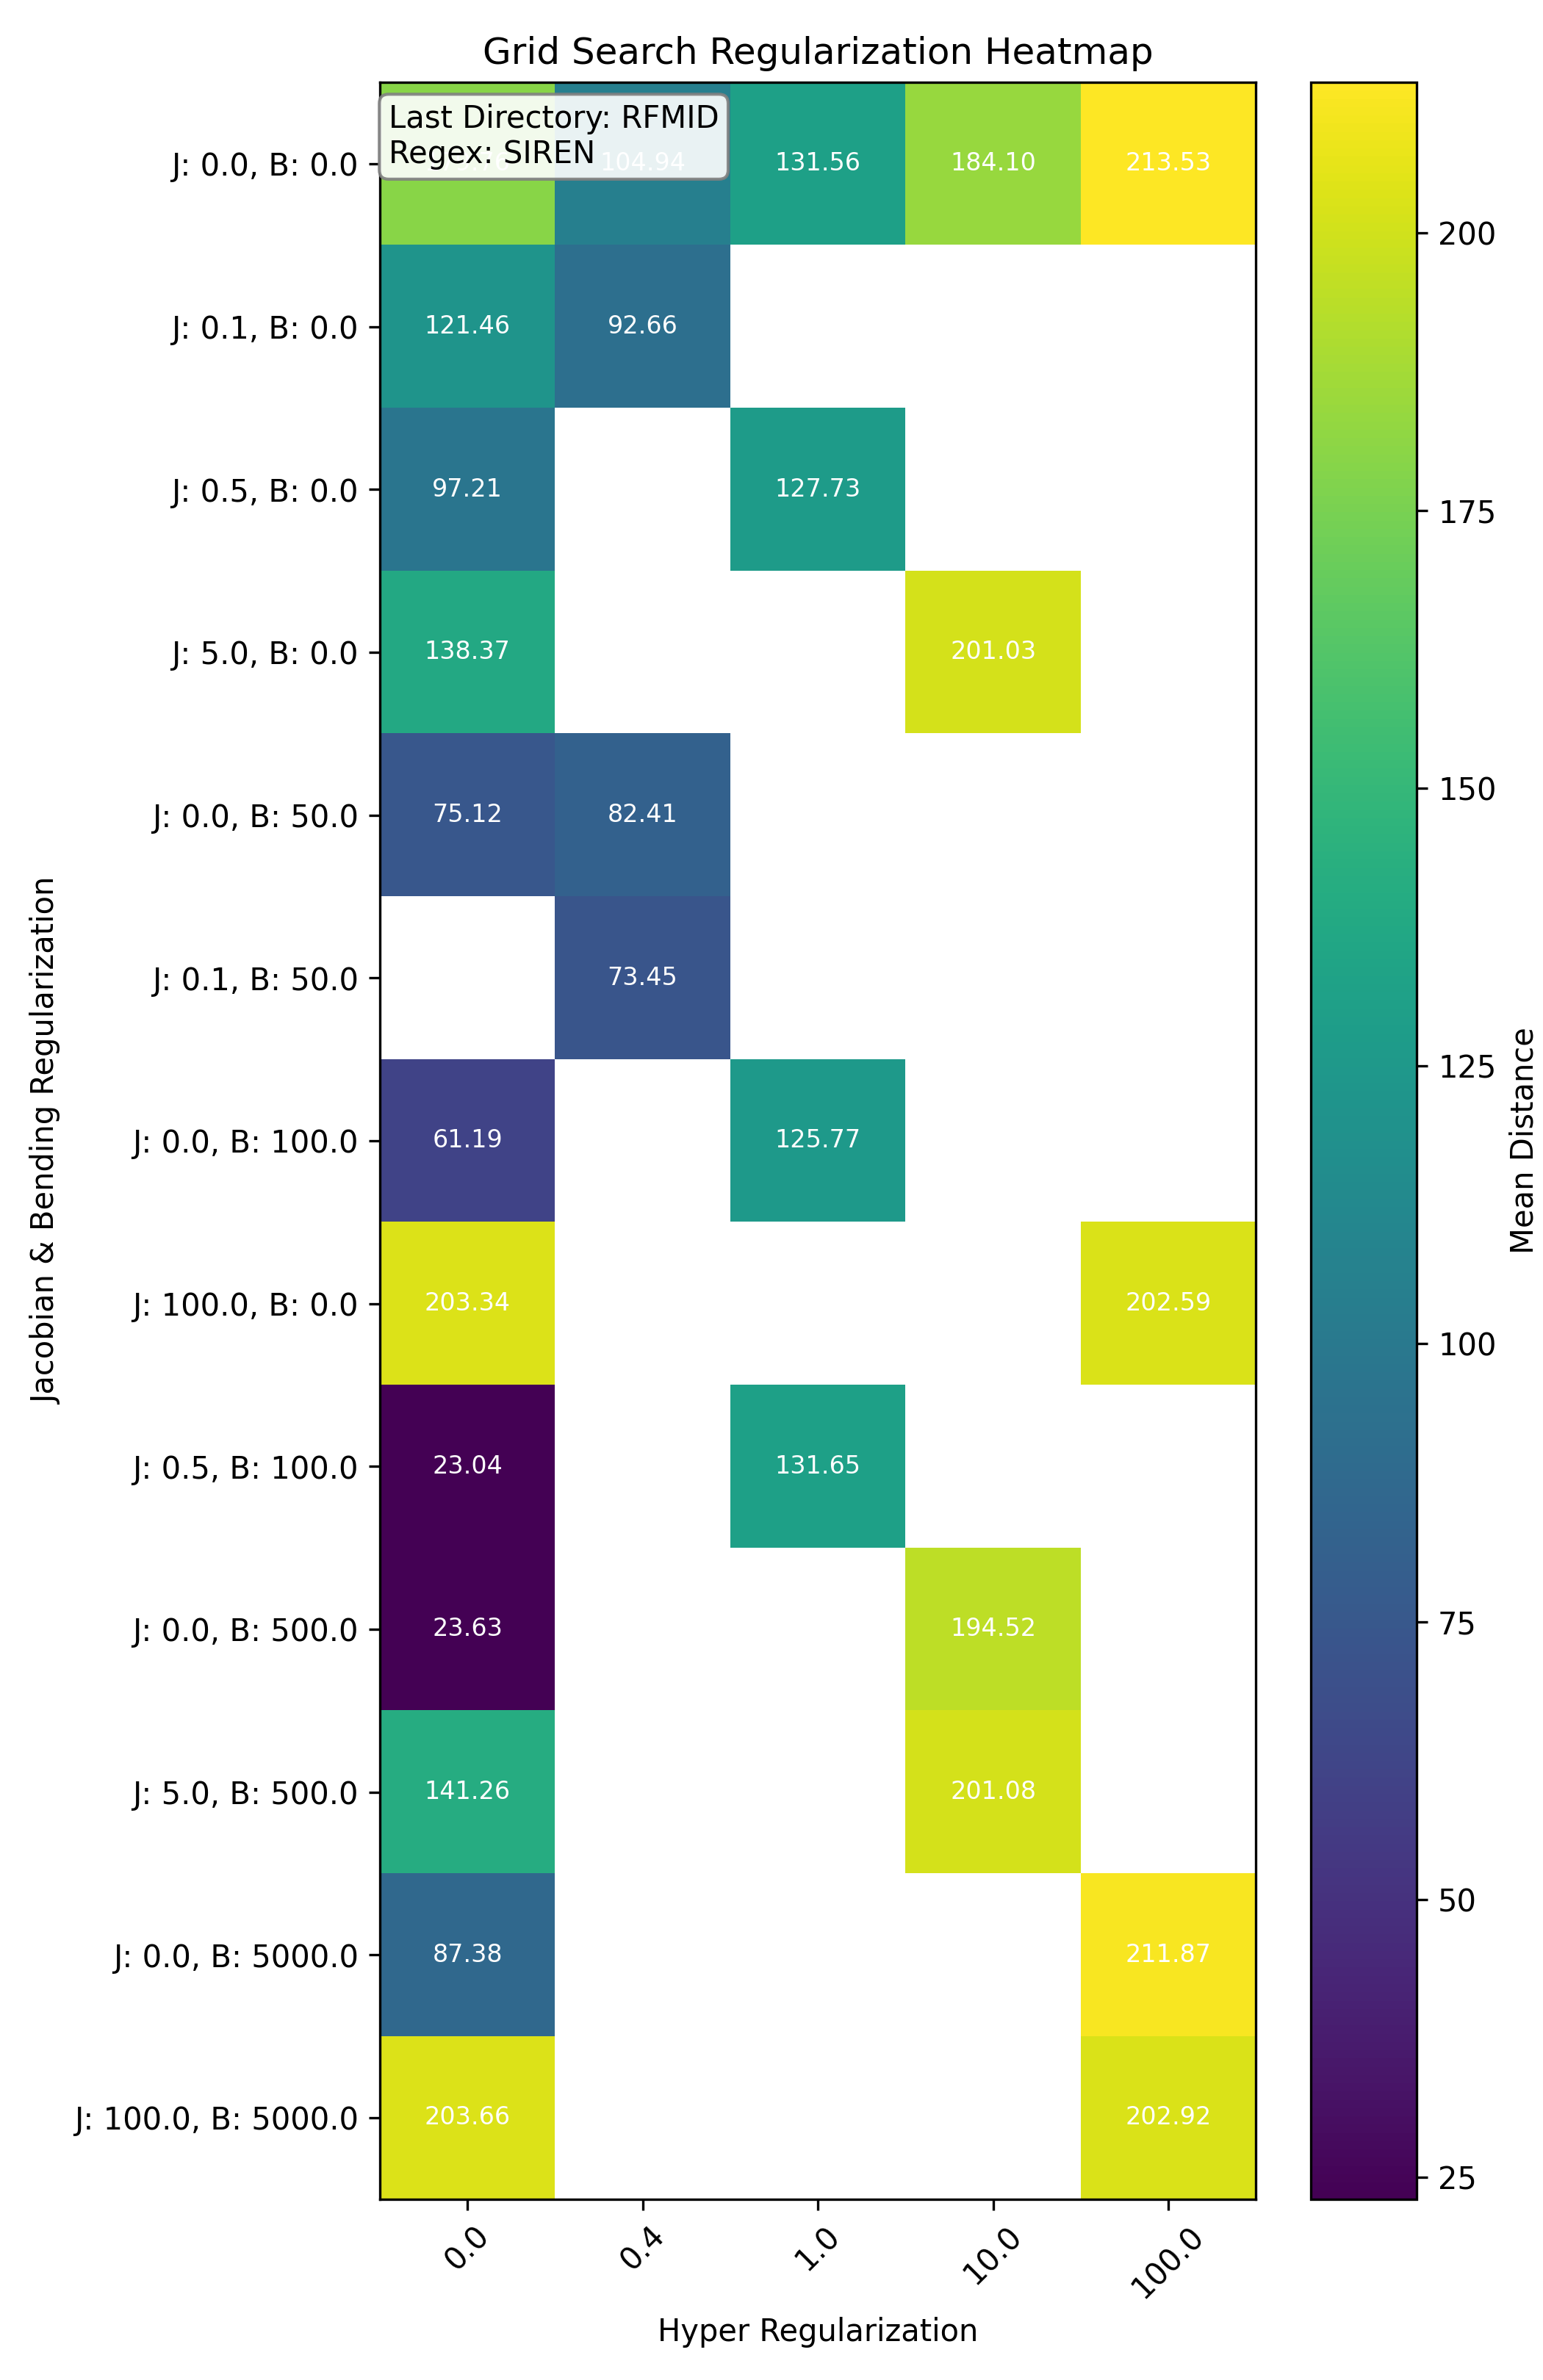
\includegraphics[width=\textwidth]{imaxes/grid_search_single_heatmap_RFMID_SIREN.png}
        \caption{RFMID - SIREN}
        \label{fig:gs_single_RFMID_SIREN}
    \end{subfigure}
    
    \caption{Single heatmap grid search results for regularization parameter tuning.}
    \label{fig:gs_single_heatmaps}
\end{figure}


\paragraph{Discusión}
\label{par:Discusión}

\paragraph{Conclusións}
\label{par:Conclusións}



\subsubsection{Learning rate}
\label{subsubsec:Learning rate}

\paragraph{Planteamento}
\label{par:Planteamento}

Debido á natureza da rede, o batch size utilzado ten unha relación directa co batch size, polo que tentaremos determinar a relación óptima entre ambos.
Ao igual que os experimentos anteriores, esta norma pode ser diferente para cada función de activación, polo que realizaremos experimentos separados para cada unha.

\paragraph{Resultados}
\label{par:Resultados}

\begin{figure}[ht]
    \centering
    \begin{subfigure}[b]{0.45\textwidth}
        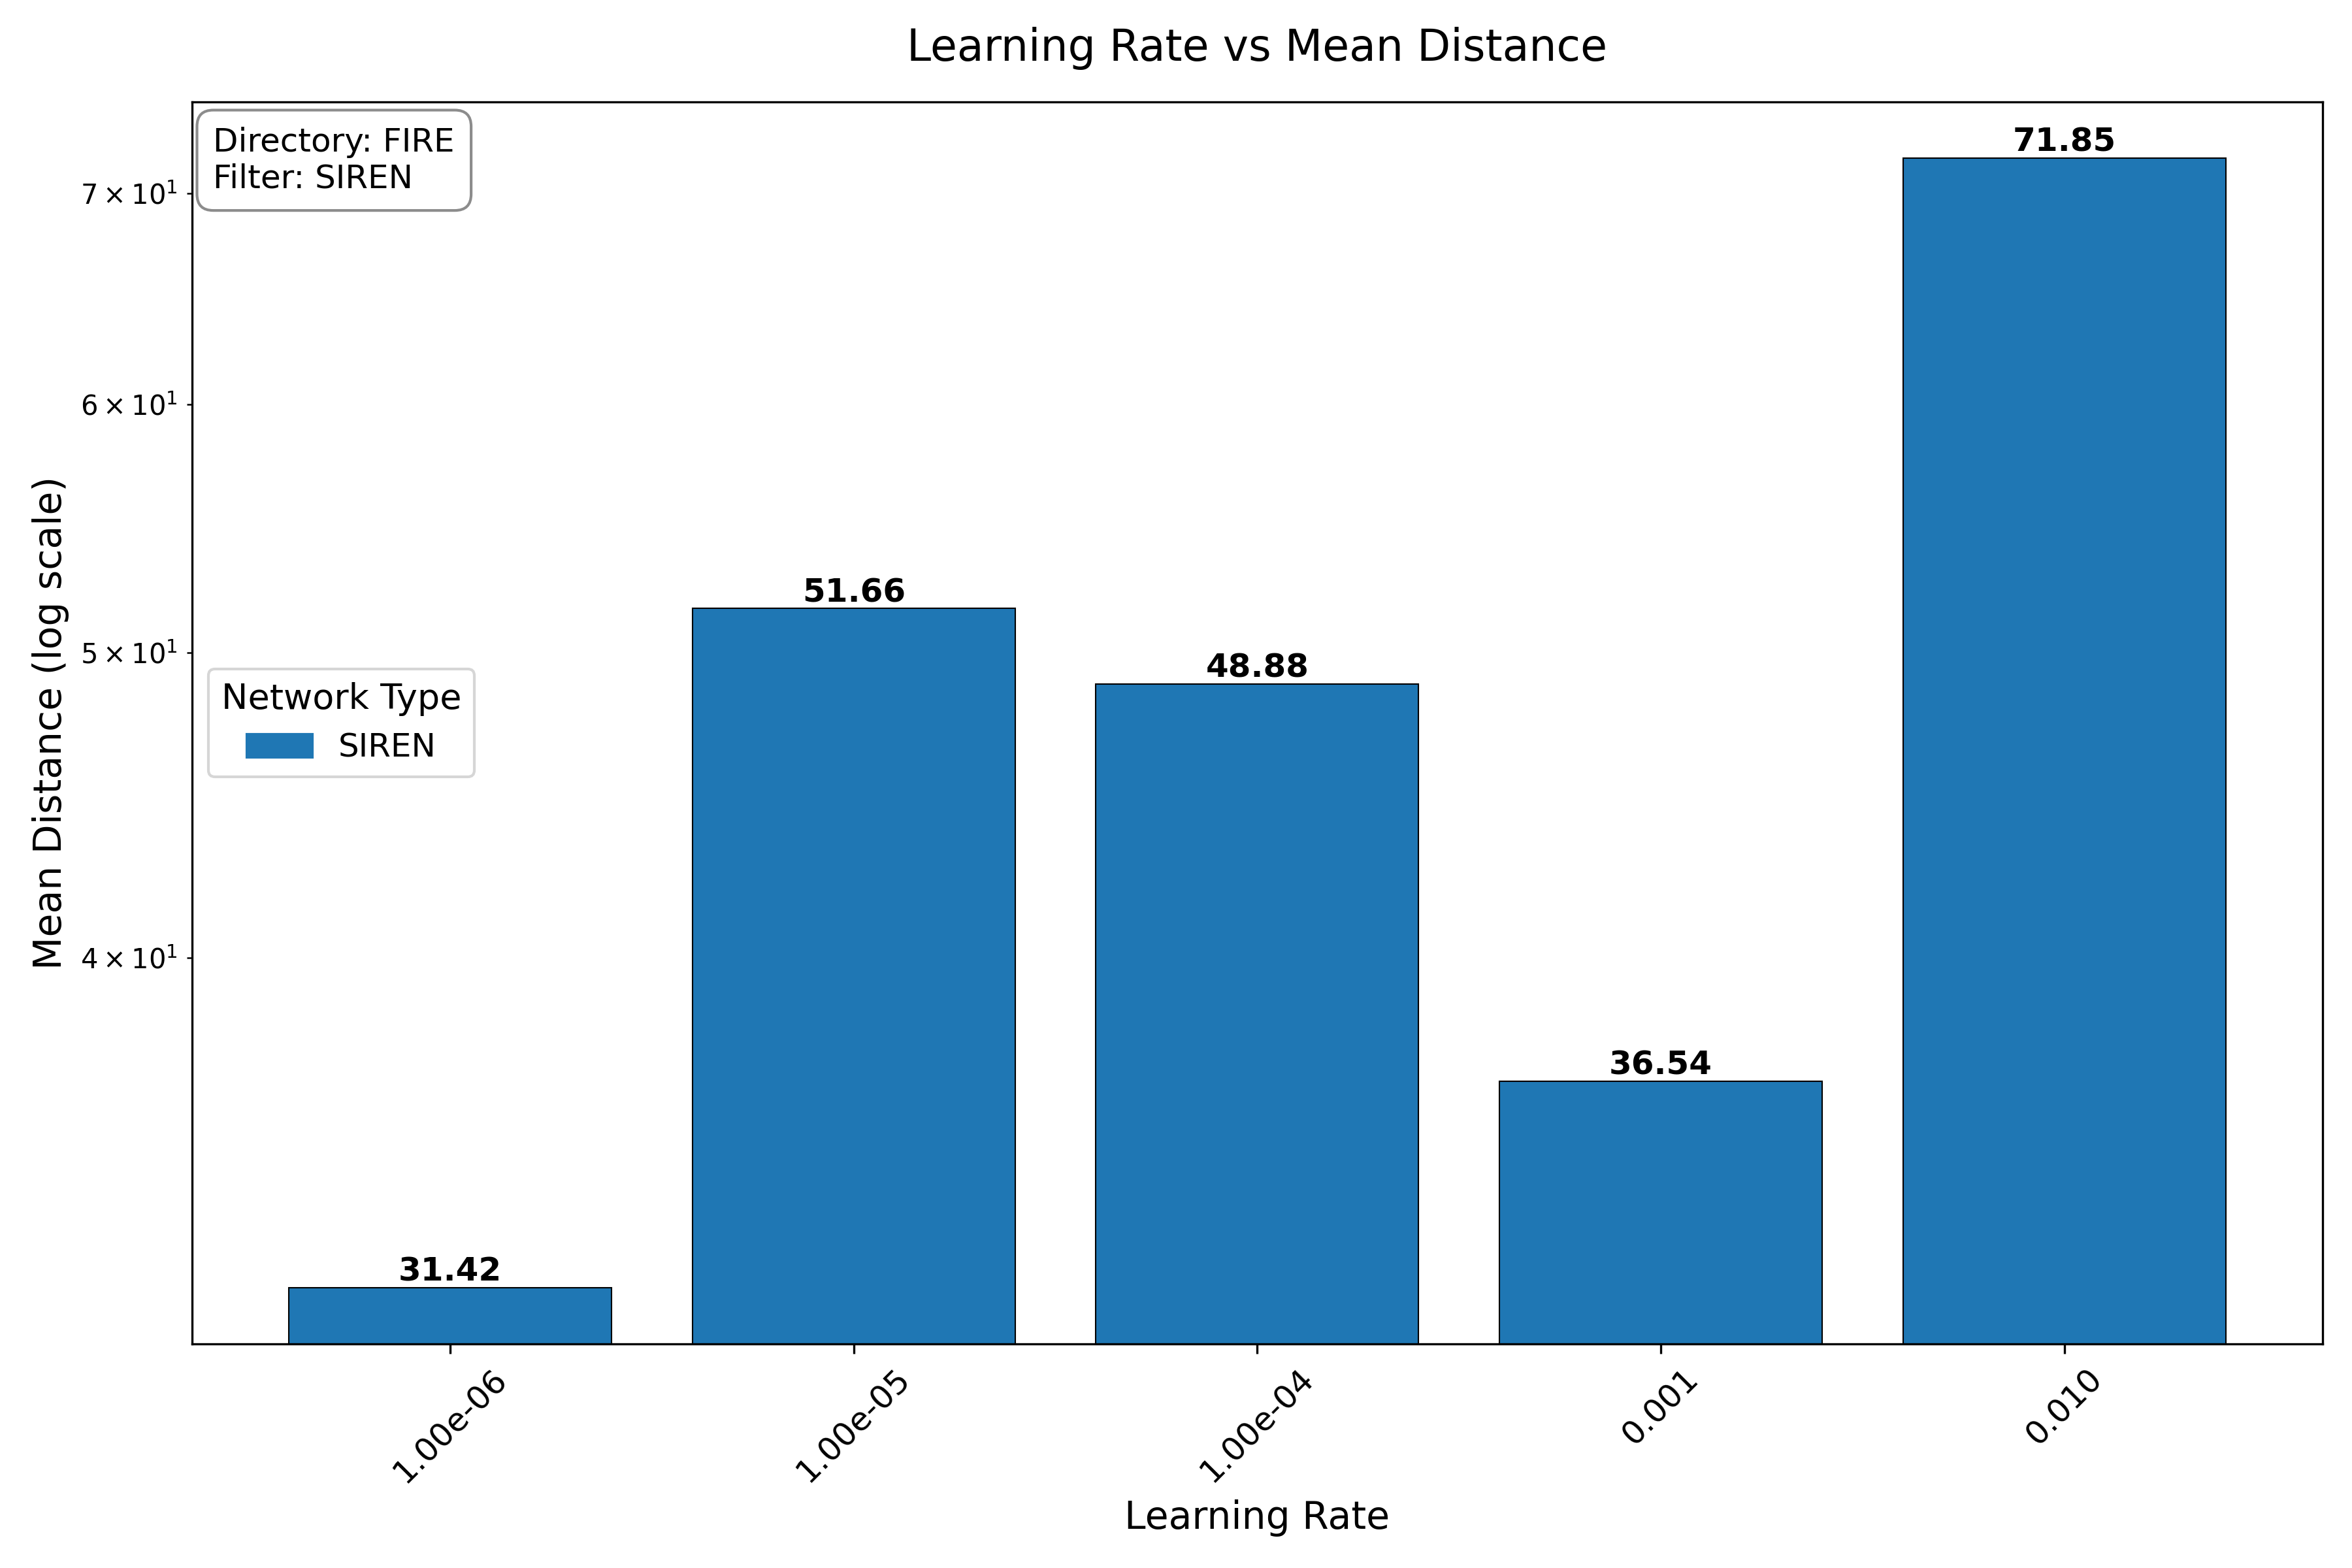
\includegraphics[width=\textwidth]{imaxes/grid_search_lr_FIRE_SIREN.png}
        \caption{FIRE - SIREN}
        \label{fig:grid_search_lr_FIRE_SIREN}
    \end{subfigure}\hfill
    \begin{subfigure}[b]{0.45\textwidth}
        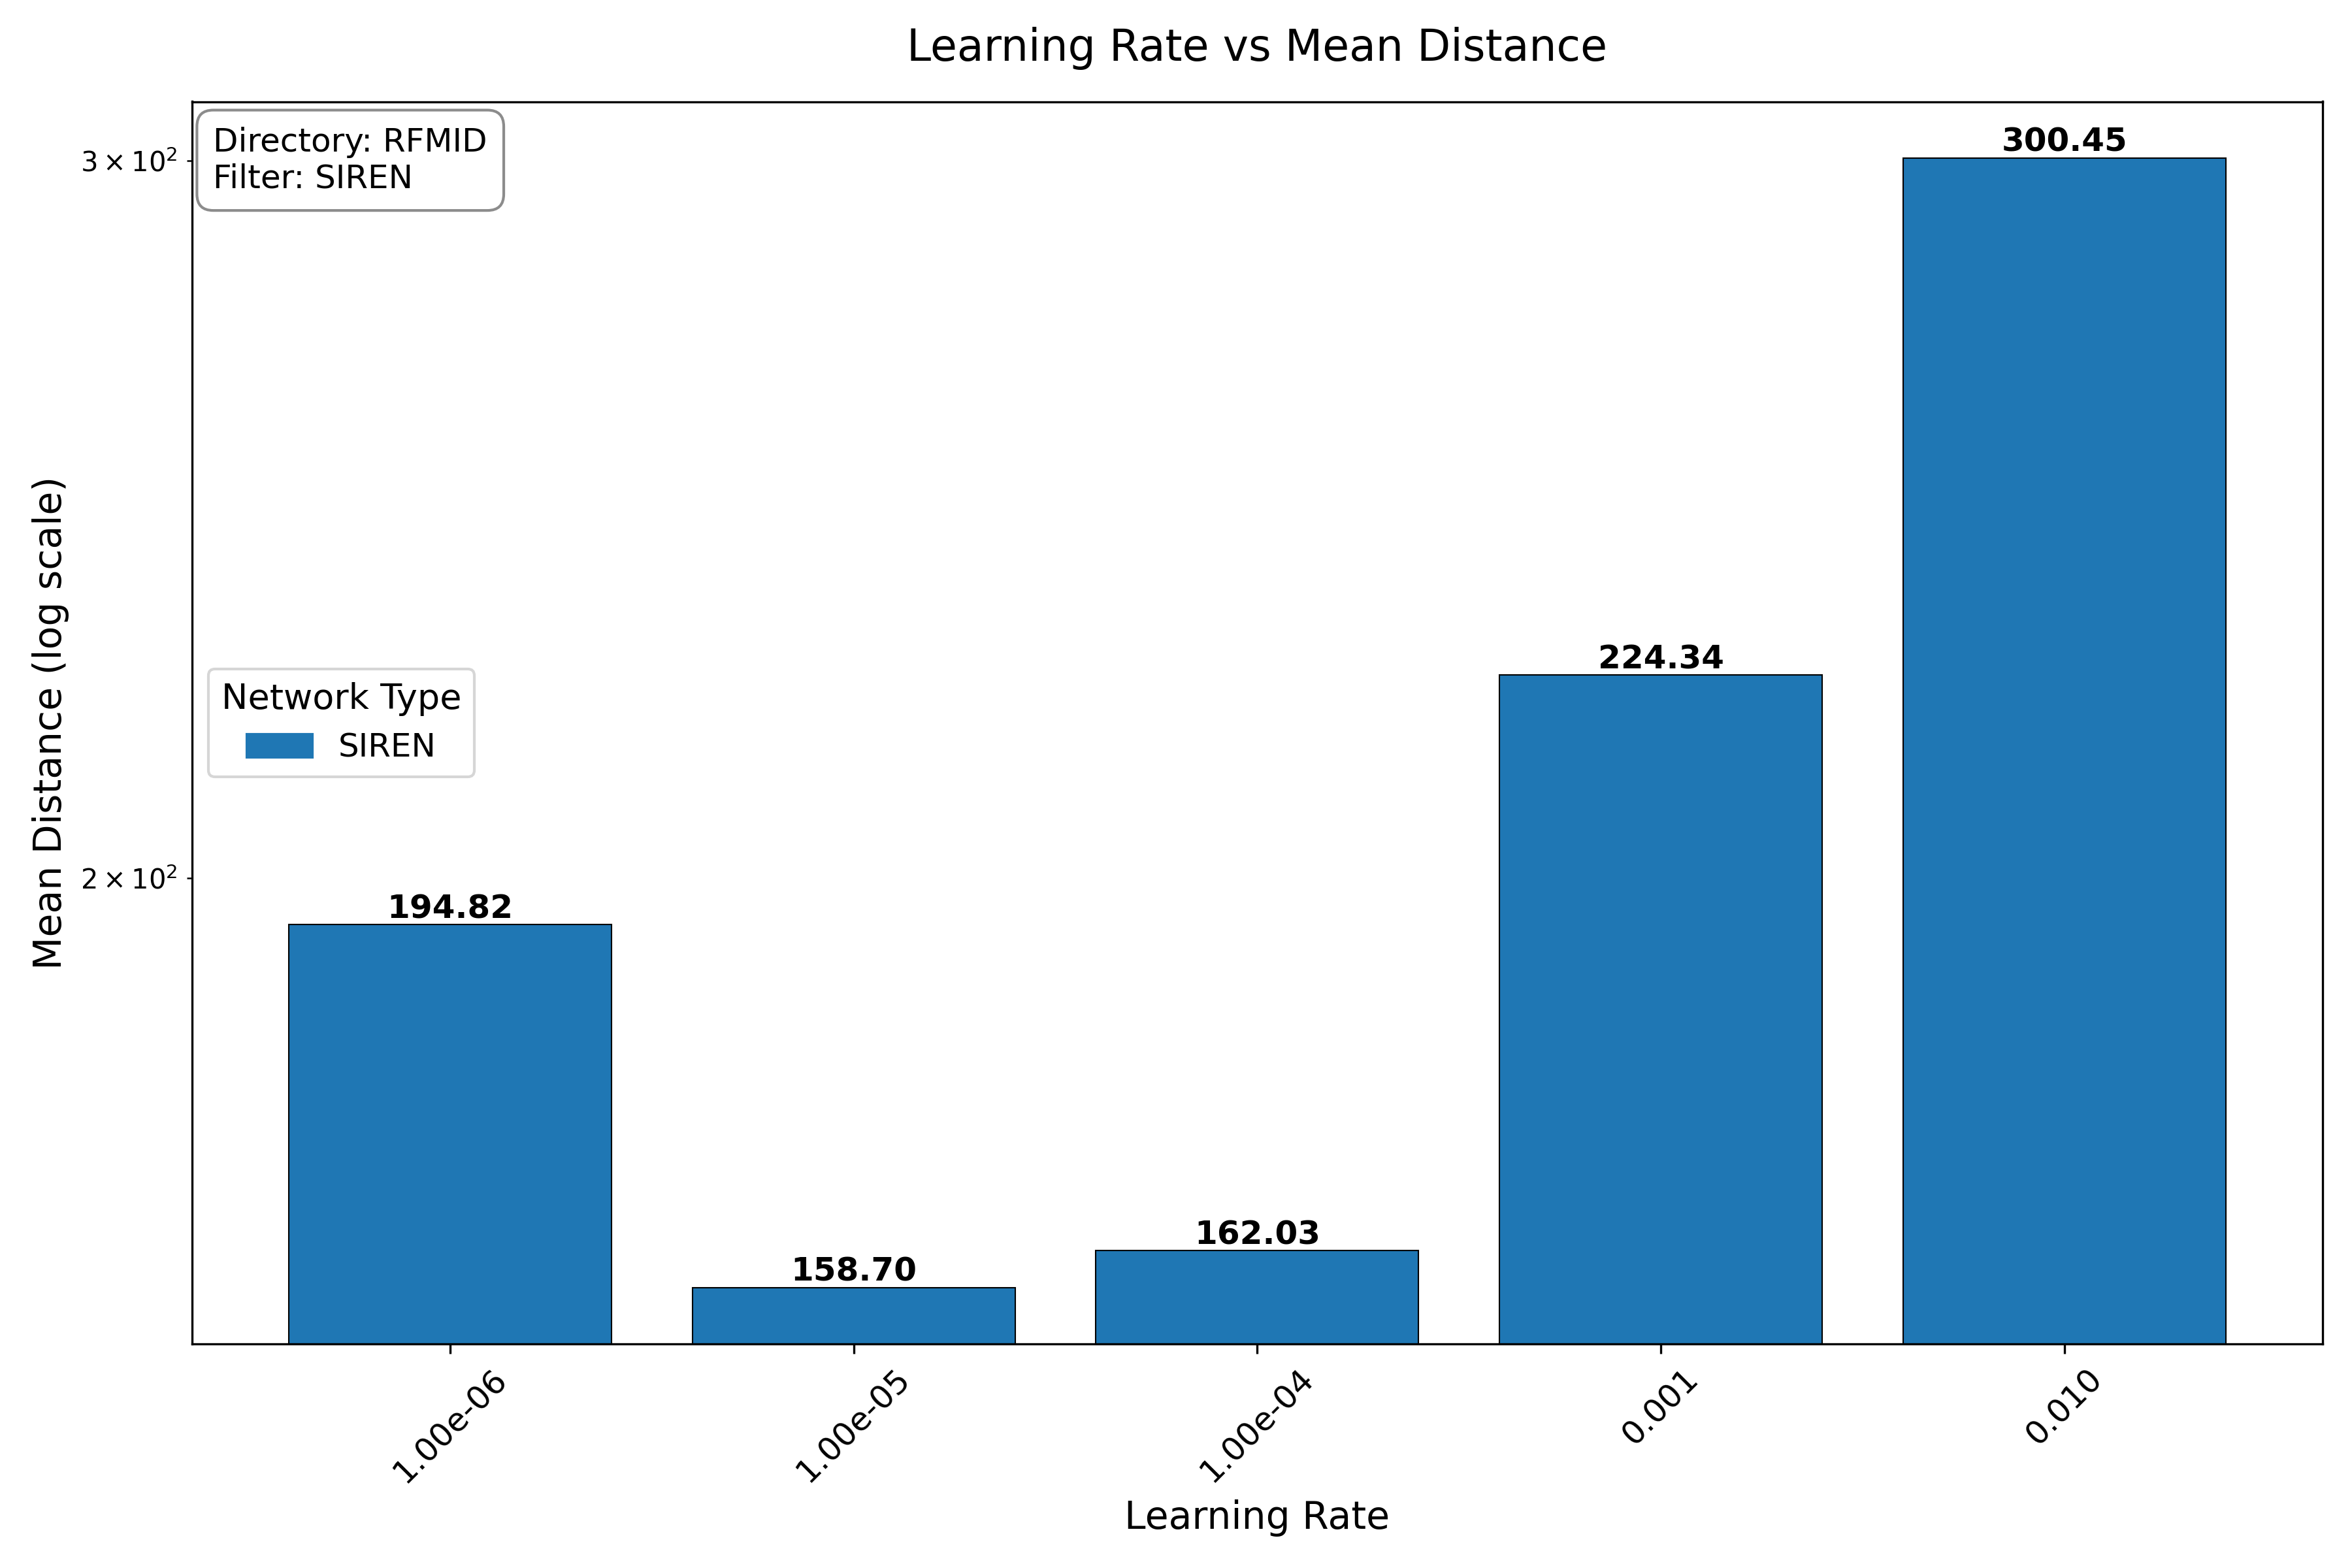
\includegraphics[width=\textwidth]{imaxes/grid_search_lr_RFMID_SIREN.png}
        \caption{RFMID - SIREN}
        \label{fig:grid_search_lr_RFMID_SIREN}
    \end{subfigure}
    \vskip\baselineskip
    \begin{subfigure}[b]{0.45\textwidth}
        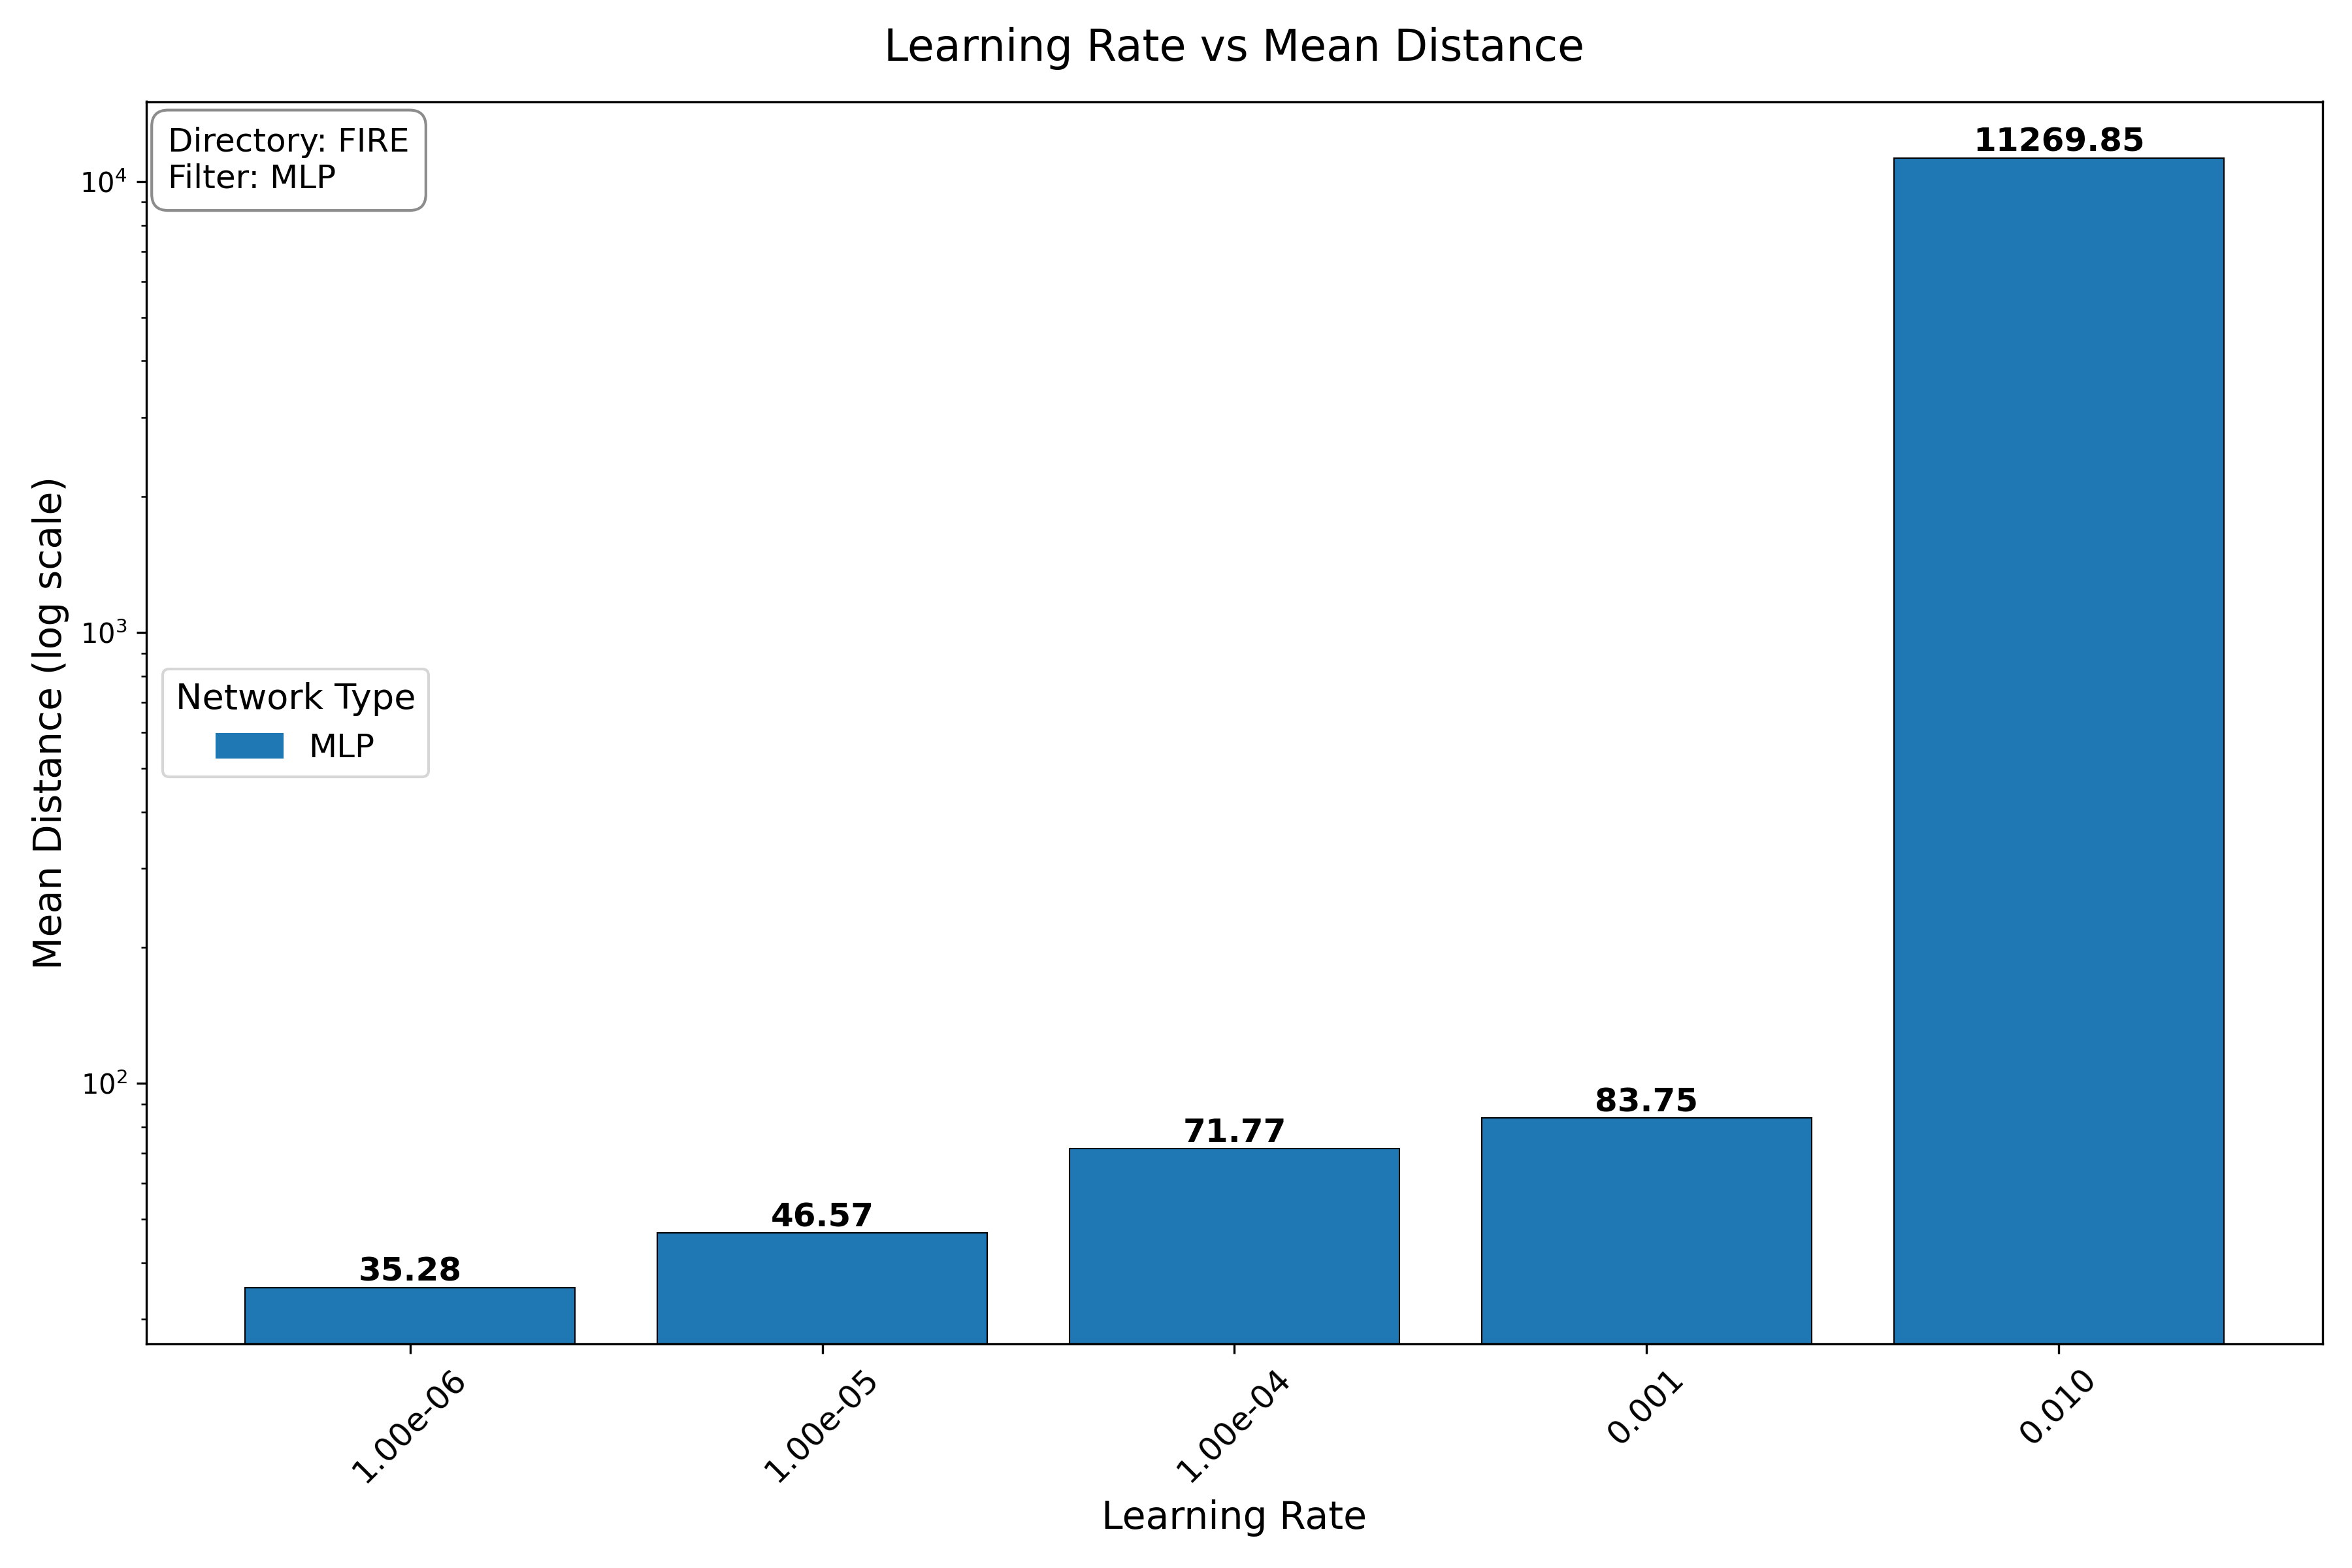
\includegraphics[width=\textwidth]{imaxes/grid_search_lr_FIRE_MLP.png}
        \caption{FIRE - Relu}
        \label{fig:grid_search_lr_FIRE_MLP}
    \end{subfigure}\hfill
    \begin{subfigure}[b]{0.45\textwidth}
        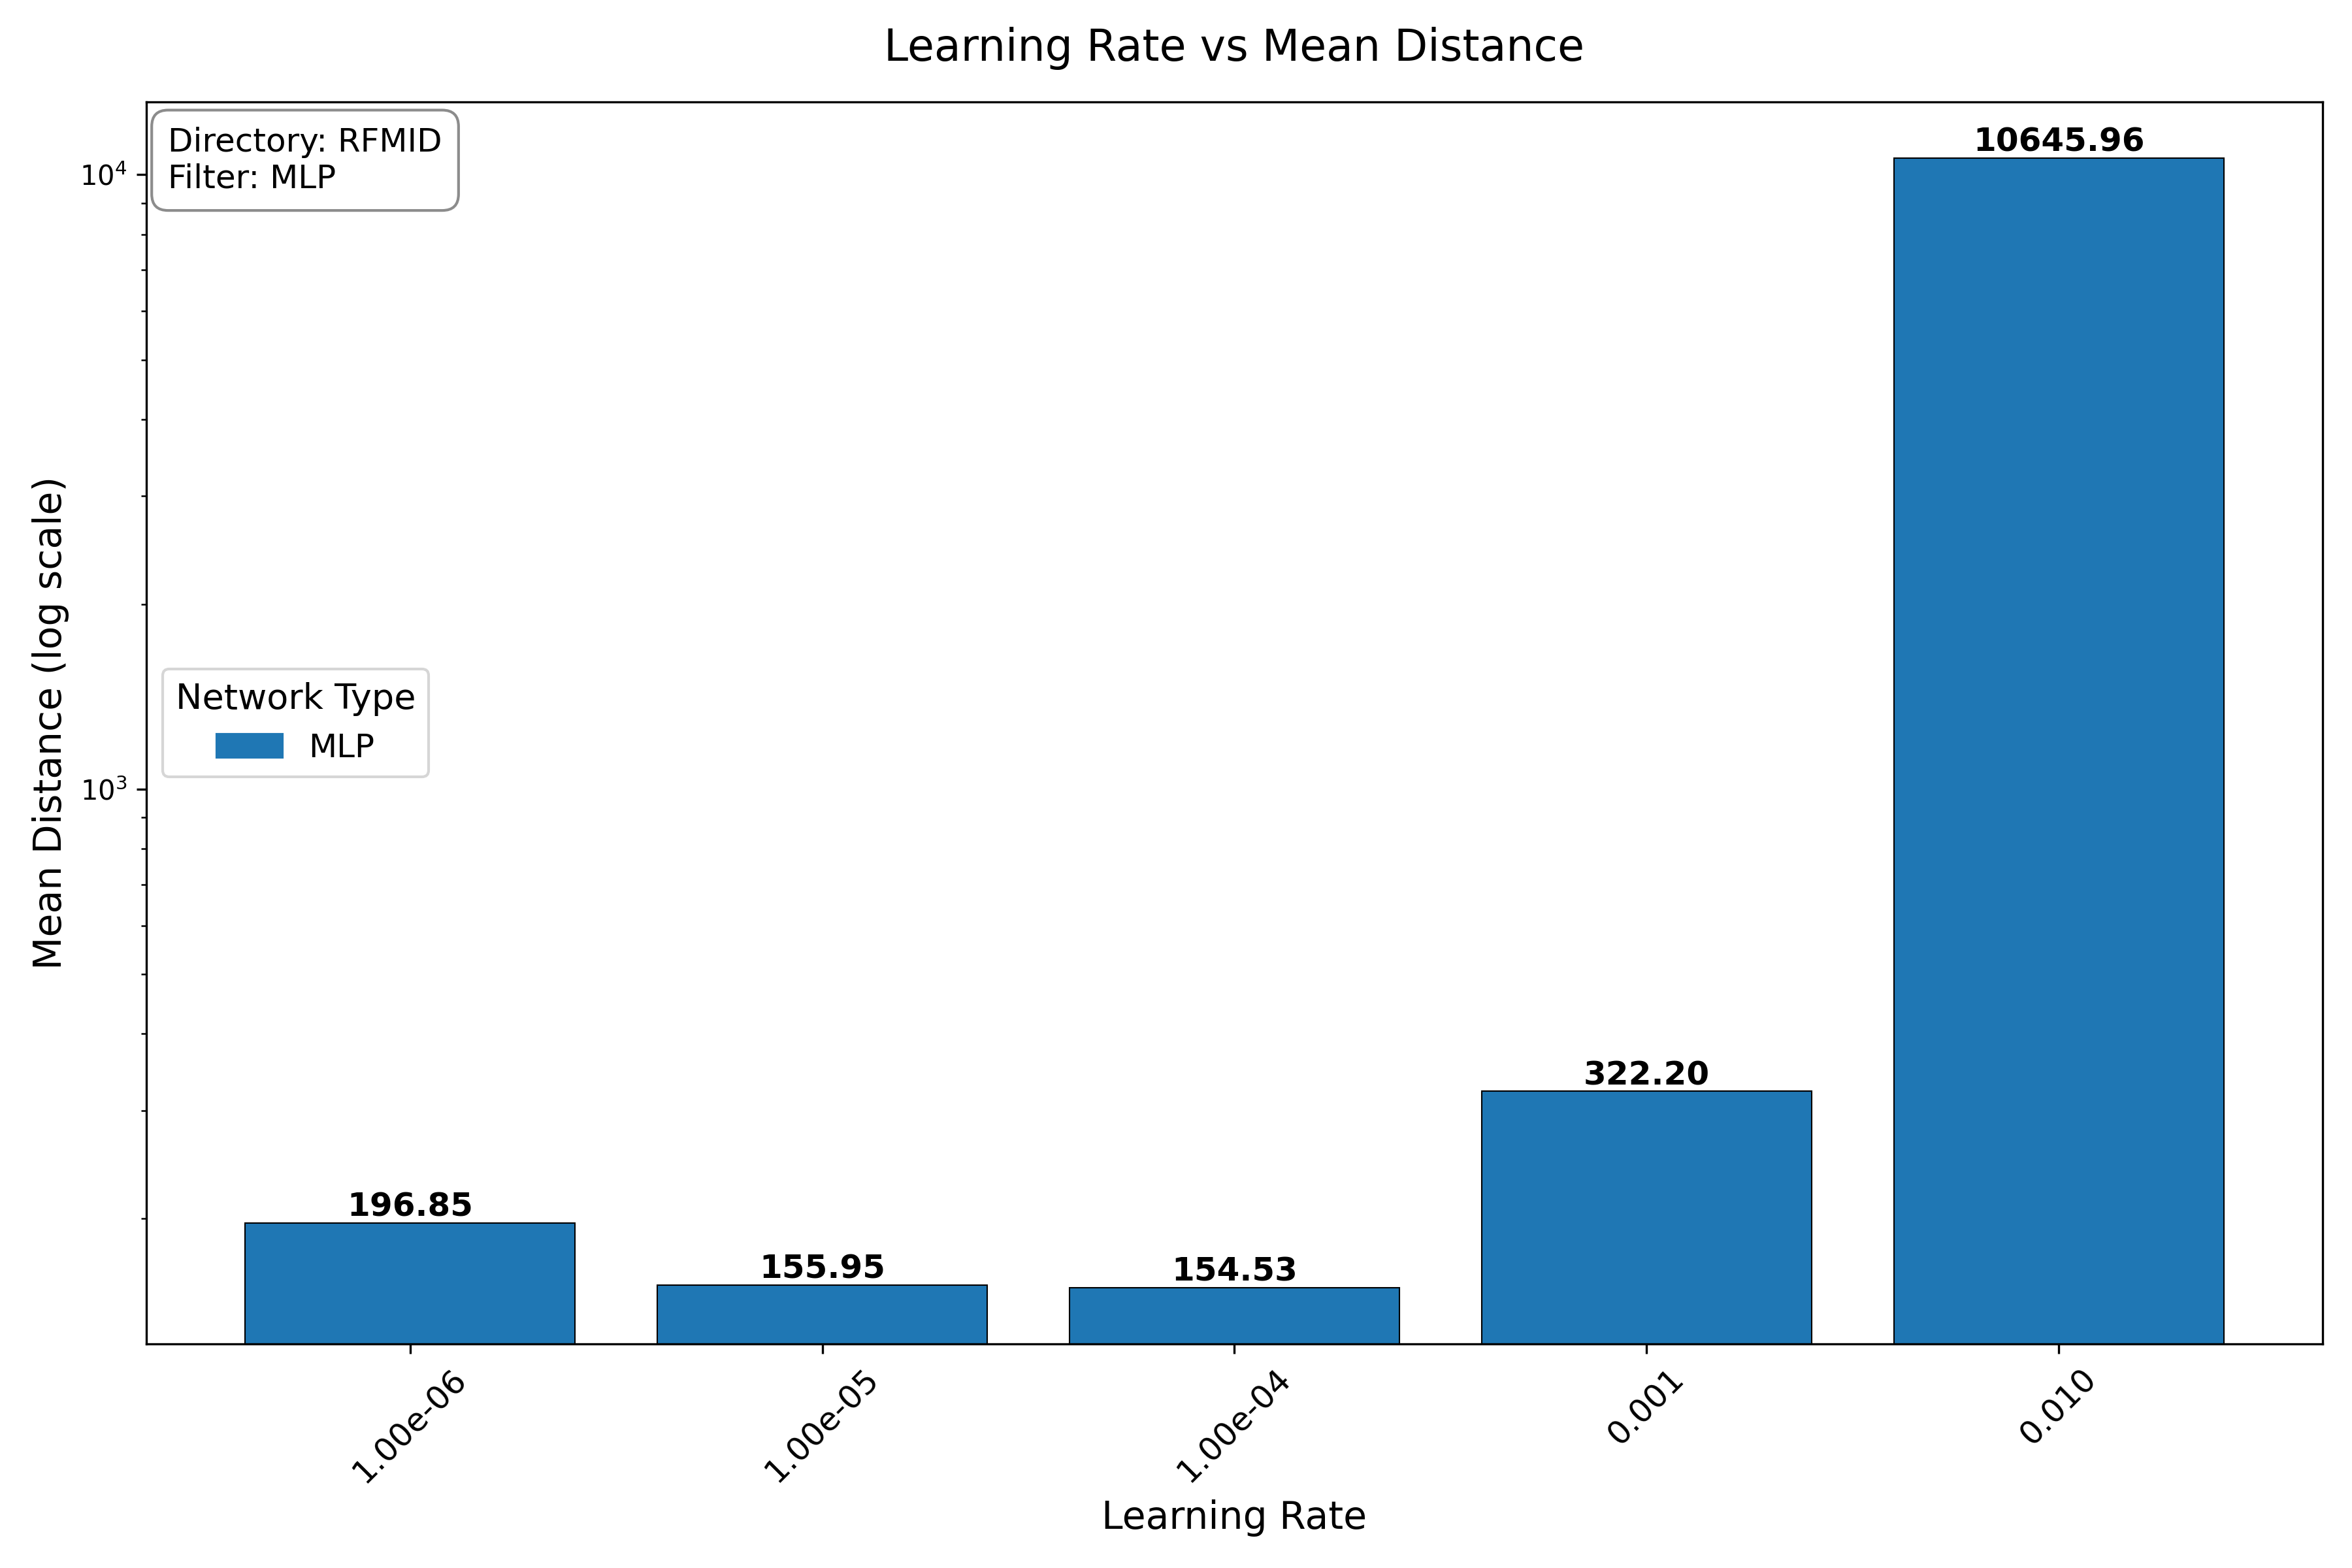
\includegraphics[width=\textwidth]{imaxes/grid_search_lr_RFMID_MLP.png}
        \caption{RFMID - Relu}
        \label{fig:grid_search_lr_RFMID_MLP}
    \end{subfigure}
    \caption{Reusltados lr cos datasets FIRE e RFMID, empregando funcións de activación SIREN e Relu.}
    \label{fig:grid_search_lr}
\end{figure}


\begin{figure}[ht]
    \centering
    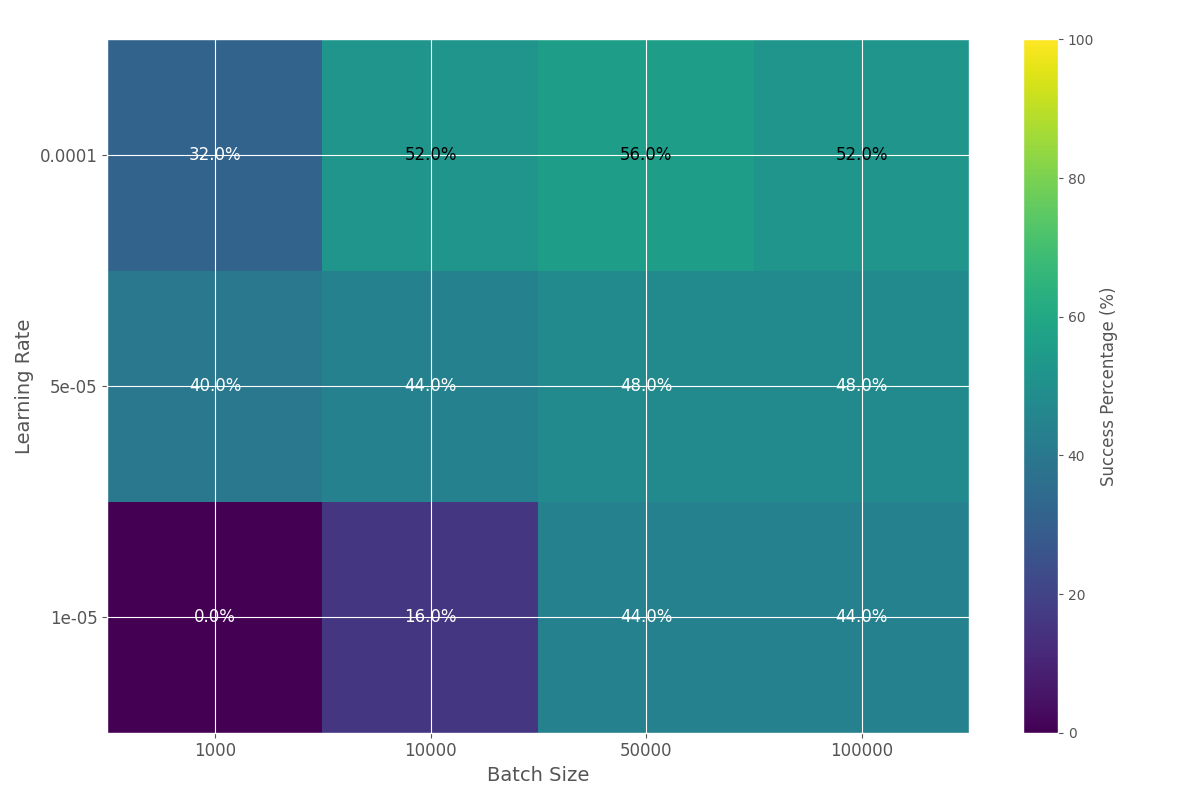
\includegraphics[width=0.8\textwidth]{imaxes/e_heatmap_MLP_RFMID.png}
    \caption{Mapa de calor cos resultados de diferentes combinacións de batch size e learning rate con unha mostra de imaxes de RMIFD ca función de activación ReLU}
    \label{fig:e_heatmap_MLP_RFMID}
\end{figure}

\paragraph{Discusión}
\label{par:Discusión}

Unha das heurísiticas mais comúns para relacionar o learning rate e o batch size é a regla de escalado linear \cite{goyal2018accuratelargeminibatchsgd}. 
A regla indica que o learning rate óptimo debe escalarse linearmente co tamaño do batch size. 

Unha forma de explicar isto é, xa que con batches mais grandes temos unha mellor aproximación do gradiente real, é posible utilizar un learning rate maior sen que a rede diverxa.


\paragraph{Conclusións}
\label{par:Conclusións}




\subsection{Batch size}
\label{subsec:Batch size}

\paragraph{Planteamento}
\label{par:Planteamento}

Ao longo dos experimentos realizados, o análisis cualitativo revelou que o batch size é un dos parámetros que máis impacto ten no rendemento da rede.
Unha vez determinados uns valores aceptables nos parámetros anteriores, realizáronse experimentos para determinar cal era o batch size óptimo.

Neste caso dividimos o conxunto de datos de RFMID en varios subconxuntos según a dificultade da transformación, medida mediante a norma de Frobenius.
Esta é unha xeralización da distancia euclidiana aplicada a matrices, desta forma as imaxes con transformacións mais grandes considéranse mais difíciles.


\paragraph{Resultados}
\label{par:Resultados}


\begin{figure}[ht]
    \centering
    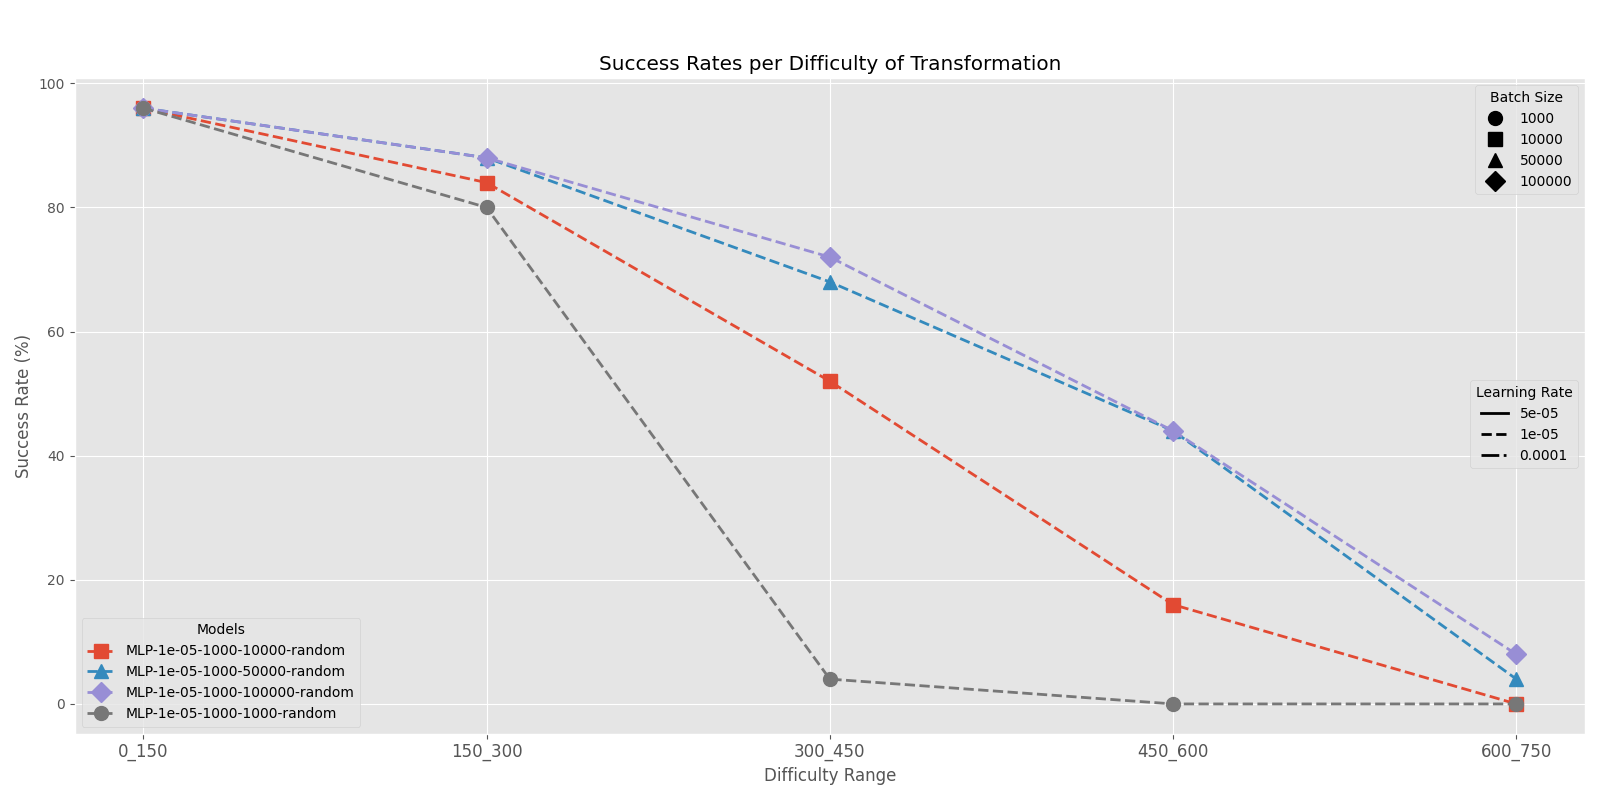
\includegraphics[width=0.8\textwidth]{imaxes/experiment_plot_RFMID_MLP_1e-05.png}
    \caption{Comparación do rendemento da rede con diferentes batch sizes sobre imaxes do dataset RFMID ca función de activación ReLU}
    \label{fig:batch_size_comparison_relu}
\end{figure}

\paragraph{Discusión}
\label{par:Discusión}

Obsérvase que un maior batch size tende a dar mellores resultados, pero a un custo computacional maior. 

\paragraph{Conclusións}
\label{par:Conclusións}

Interesa determinar cal é o punto de inflexión onde o aumento do batch size non compensa o aumento do rendemento.

\subsection{Estratexias de mostraxe}
\label{subsec:Estratexias de mostraxe}

Orixinalmente IDIR utiliza unha estratexia de mostraxe aleatoria para seleccionar os puntos que se pasan á rede en cada iteración.
Mentres que esta estratexia parece suficiente para o rexitro de pulmóns, no caso das imaxes de retina isto non ten porque ser así.
Isto débese a que as imaxes de retina teñen seccións con moita mais información que outras, frente os CTs de pulmóns onde o sinal é mais uniforme.
Ademais, as retinografías teñen desprazamentos moito maiores e menor superposición entre cada parella. 

\paragraph{Planteamento}
\label{par:Planteamento}

Para solucionar isto, propúxose unha estratexia de mostraxe mais intellixente, onde se calcula unha máscara de probabilidade para cada imaxe, que se utiliza para seleccionar os puntos que se pasan á rede.
Para calcular esta máscara, extráense mediante operadores de Sobel os vasos sanguíneos e mediante umbralización o disco óptico, que son as zonas onde se espera que haxa máis información, e dáselles maiores probabilidades de ser seleccionadas.
Esta aproximación estaba errada, \dots

Posteriormente probouse unha estratexia de mostraxe uniforme, onde se seleccionan un número fixo de puntos en cada imaxe, independentemente da información que conteña.
É unha estratexia similar ao mostraxe aleatorio, pero garantindo que se cubre a maior parte posible da imaxe. Isto é relevante en experimentos con batch sizes pequenos onde unha mostraxe aleatoria non ten por que cubrir toda a imaxe.
Para implementalo useouse \dots 
Fibonacci lattice points in polar form place points on a circle by assigning each point a radius (sqrt i / N) and an angle (2πi / φ²)

Así mesmo implementouse un scheduling do batch size, coa intención de utilizar poucos puntos inicialmente para que a rede aprenda unha transformación global a grandes rasgos, e aumentar o número de puntos conforme avanzase o entrenamento para que a rede aprenda as transformación locais.
A estratexia de mostraxe uniforme é a mais axeitada para este caso, especialmente cando se utiliza un batch size pequeno.

\begin{figure}[]
    \centering
    \begin{subfigure}[b]{0.3\textwidth}
        \centering
        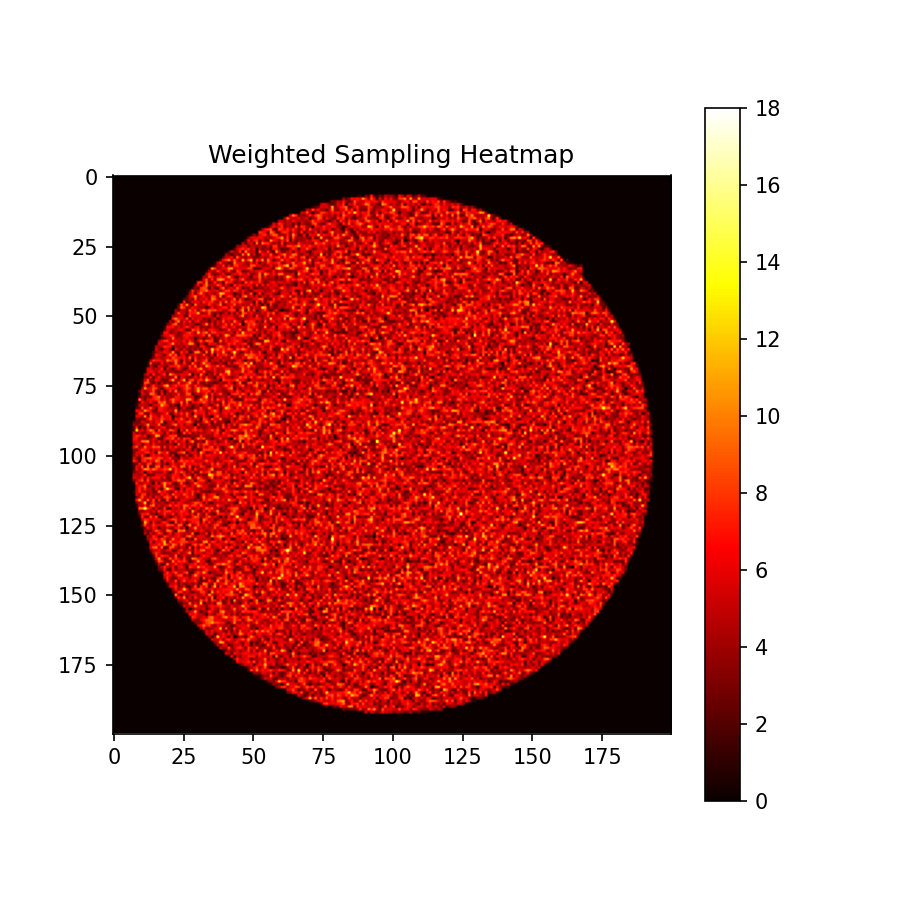
\includegraphics[width=\textwidth]{imaxes/random_sampling_heatmap.png}
        \caption{Heatmap de mostraxe aleatorio}
        \label{fig:random_sampling_heatmap}
    \end{subfigure}
    \hfill
    \begin{subfigure}[b]{0.3\textwidth}
        \centering
        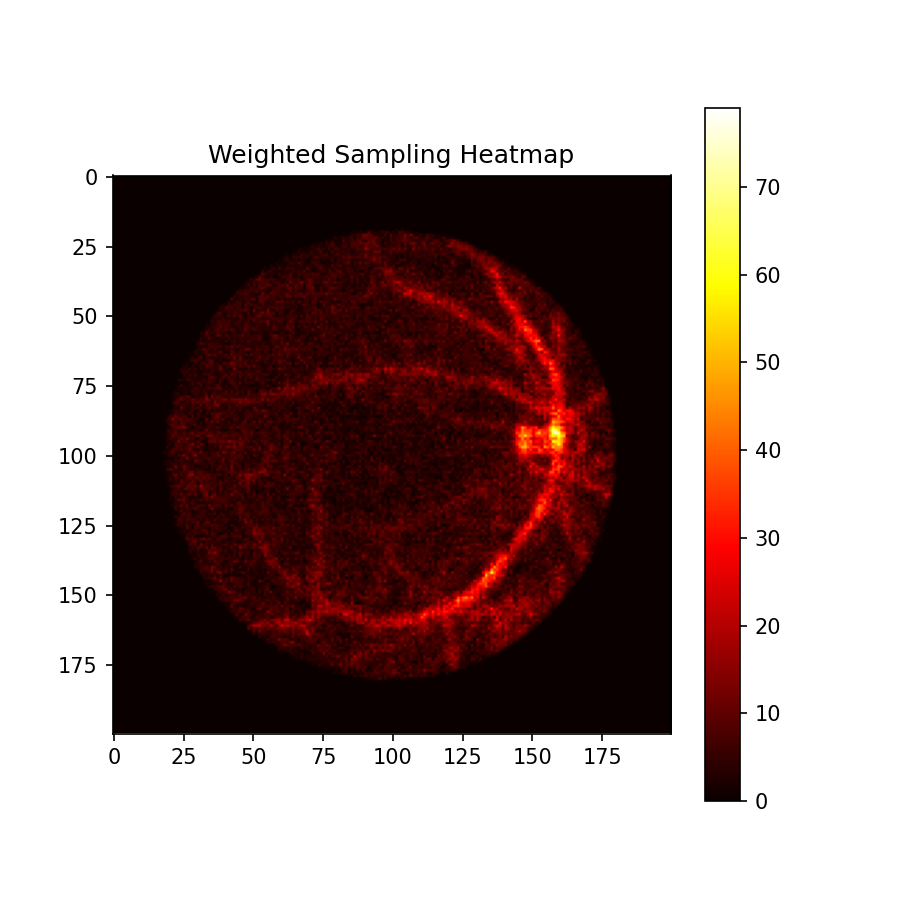
\includegraphics[width=\textwidth]{imaxes/weighted_sampling_heatmap.png}
        \caption{Heatmap de mostraxe con peso}
        \label{fig:weighted_sampling_heatmap}
    \end{subfigure}
    \hfill
    \begin{subfigure}[b]{0.3\textwidth}
        \centering
        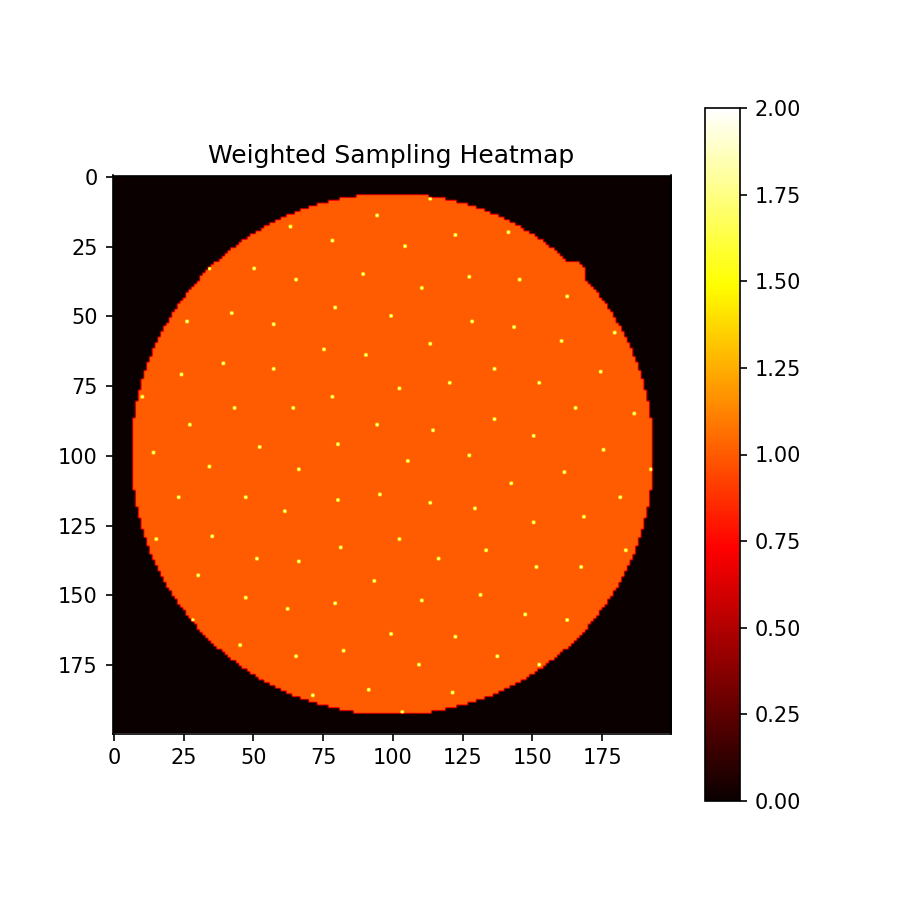
\includegraphics[width=\textwidth]{imaxes/uniform_sampling_heatmap.png}
        \caption{Heatmap de mostraxe uniforme (100 puntos)}
        \label{fig:uniform_sampling_heatmap}
    \end{subfigure}
    \caption{Heatmaps de mostraxe}
    \label{fig:sampling_heatmaps}
\end{figure}


\paragraph{Resultados}
\label{par:Resultados}


\begin{figure}[ht]
    \centering
    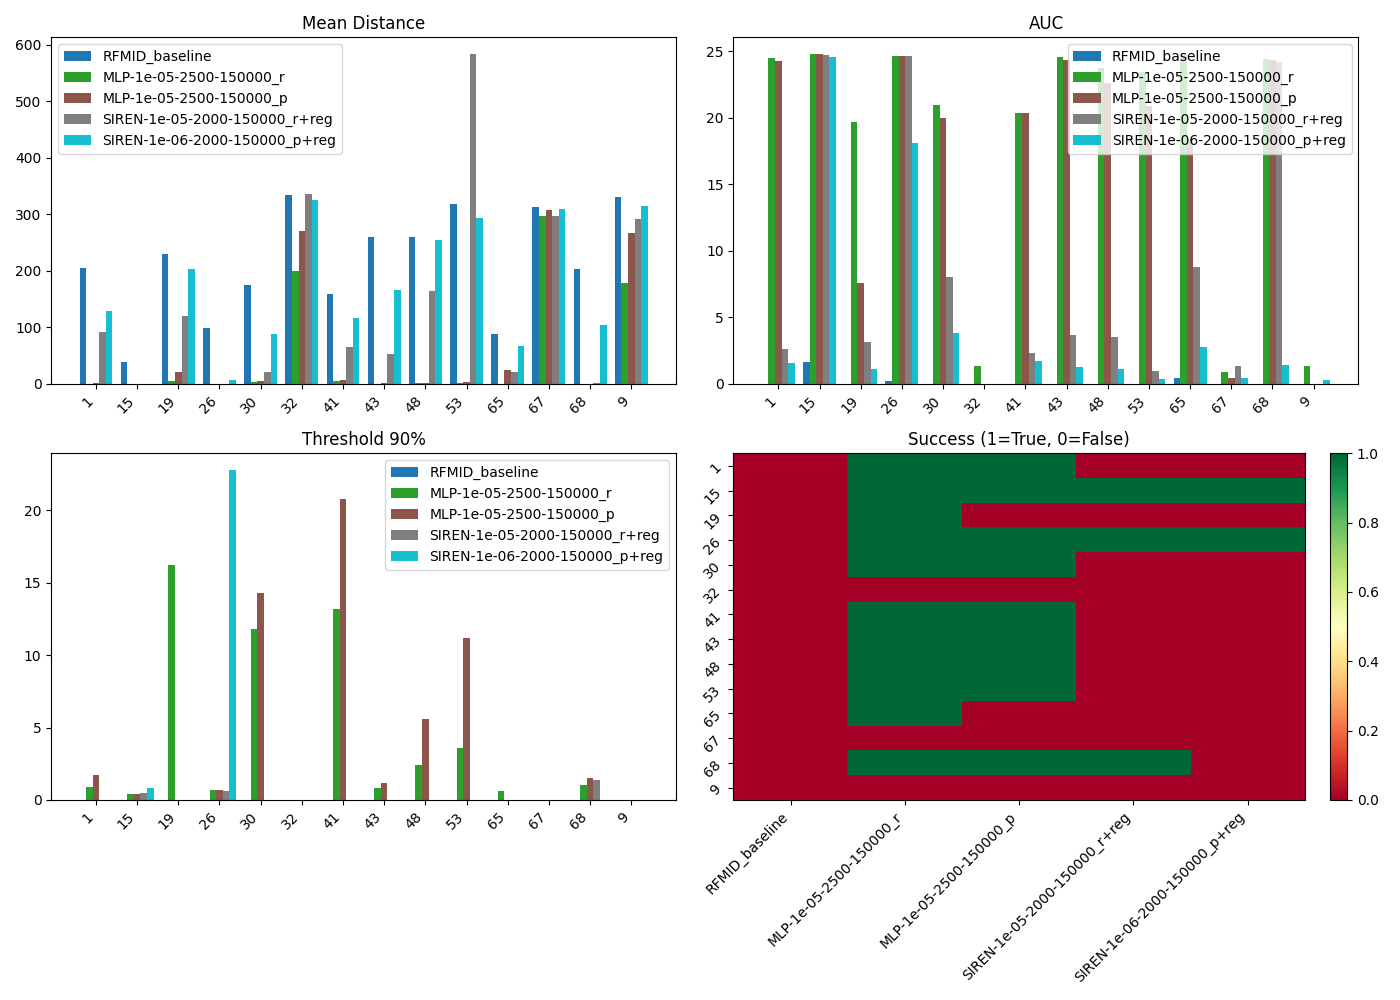
\includegraphics[width=0.8\textwidth]{imaxes/RFMID_both__comp_sampling.png}
    \caption{Comparación das diferentes estratexias de mostraxe sobre imaxes do dataset RFMID}
    \label{fig:sampling_comparison}
\end{figure}

Tamén variando o learning rate.

\begin{figure}[ht]
    \centering
    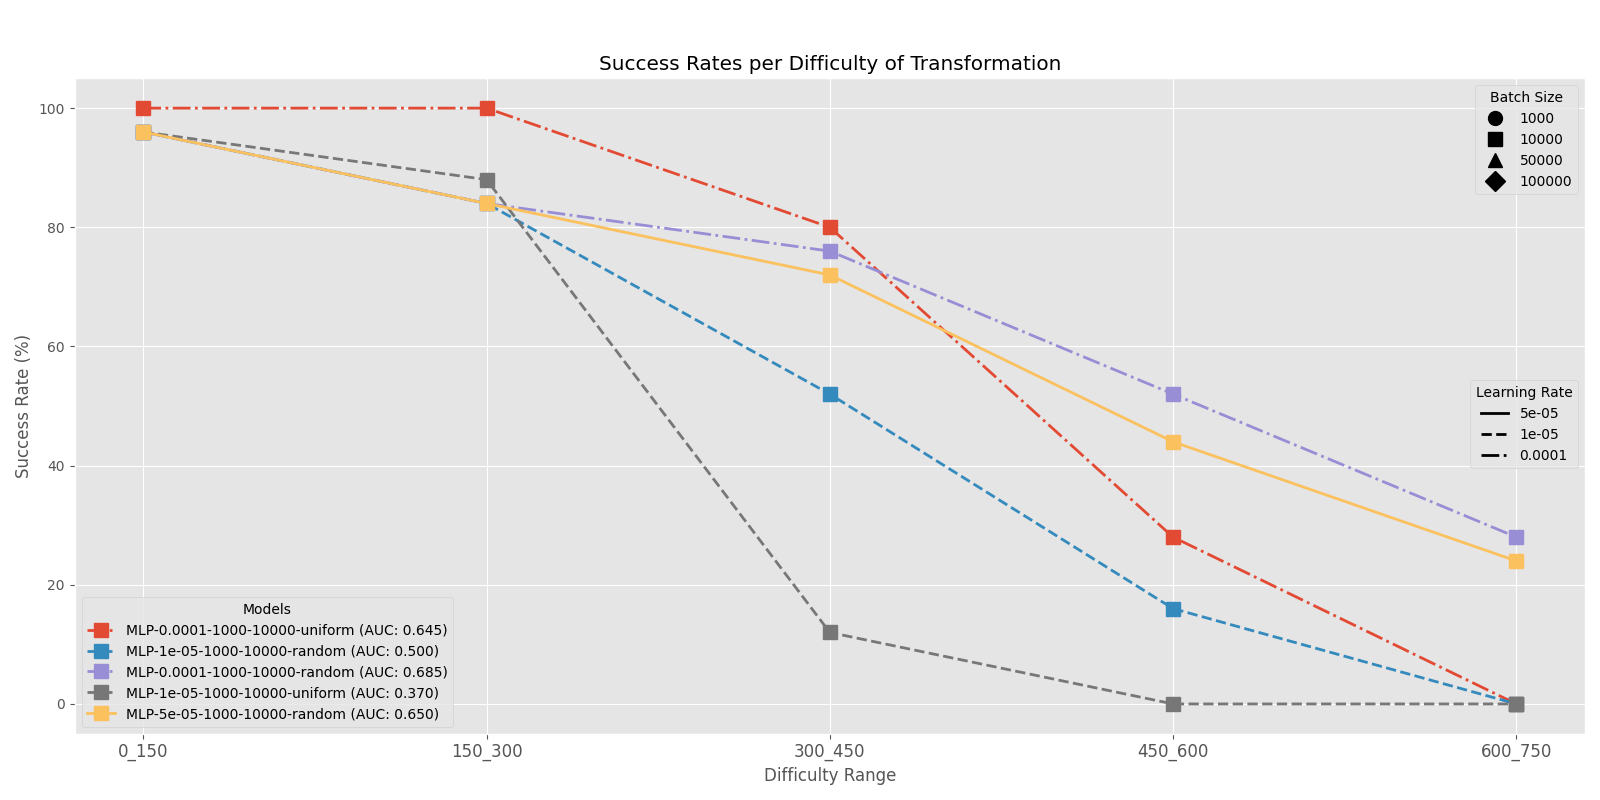
\includegraphics[width=0.8\textwidth]{imaxes/experiment_plot_RFMID_MLP_RvsU.png}
    \caption{Comparación das diferentes estratexias de mostraxe sobre imaxes do dataset RFMID ca función de activación RELU}
    \label{fig:sampling_comparison_relu}
\end{figure}

\begin{figure}[ht]
    \centering
    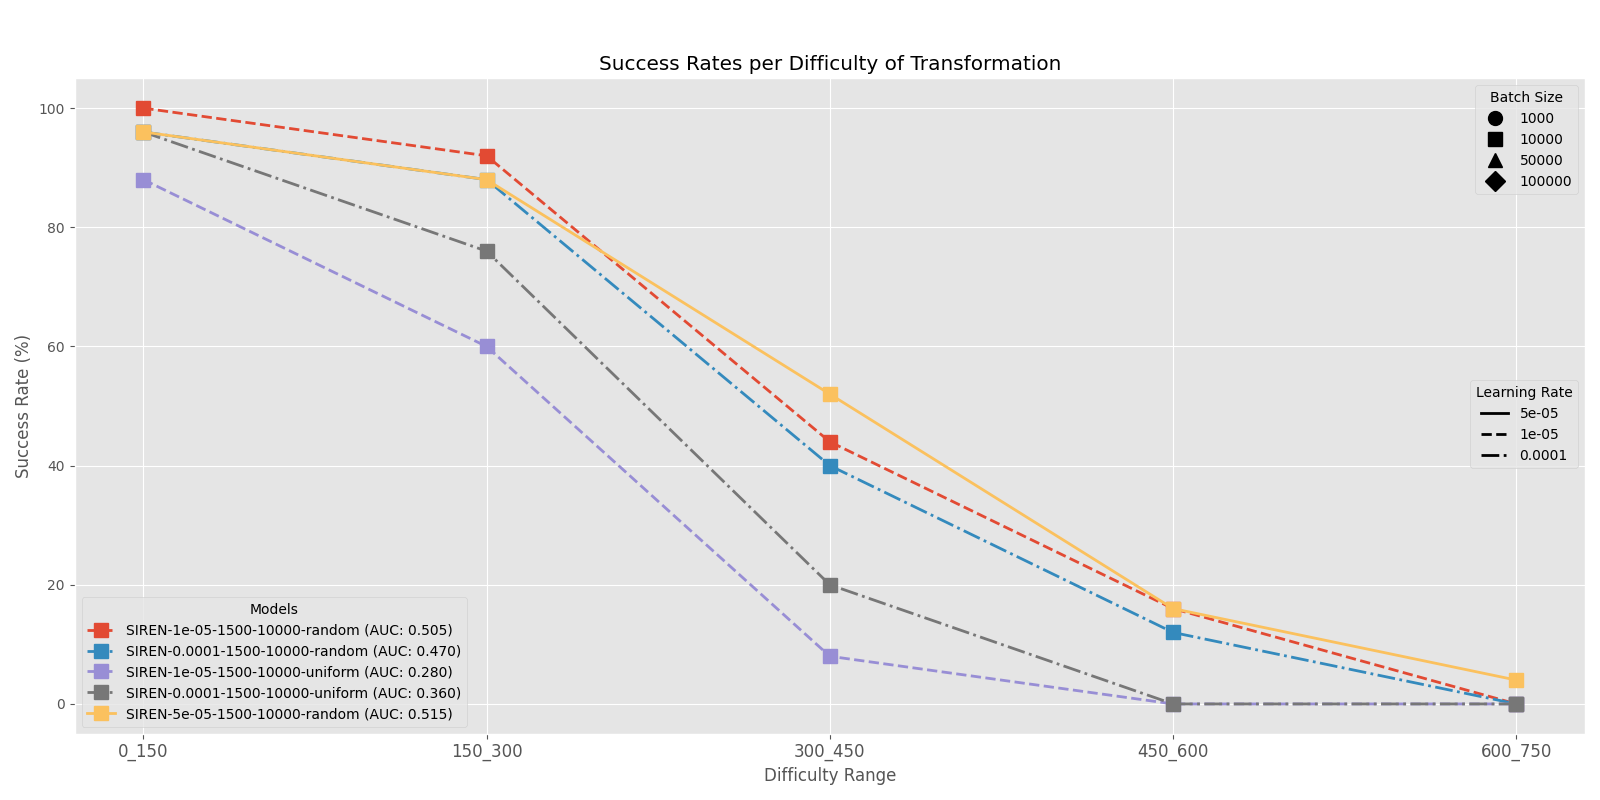
\includegraphics[width=0.8\textwidth]{imaxes/experiment_plot_RFMID_SIREN_RvsU.png}
    \caption{Comparación das diferentes estratexias de mostraxe sobre imaxes do dataset RFMID ca función de activación SIREN}
    \label{fig:sampling_comparison_SIREN}
\end{figure}

Falar da implementación de cada tipo...


\paragraph{Discusión}
\label{par:Discusión}

A hipótese inicial era que a estratexia de mostraxe con peso sería a mais axeitada, xa que se seleccionan máis puntos nas zonas onde se espera que haxa máis información.
Non obstante, os resultados 

\paragraph{Conclusións}
\label{par:Conclusións}

\subsection{Inicialización}
\label{subsec:Inicialización}

É posible que a inicialización da rede sexa un factor mais importante que a estratexia de mostraxe\dots

Implementouse unha lotería de inicialización, onde se utiliza o loss no epoch 0 para determinar a inicialización da rede mais beneficiosa.
É posible que fore mellor esperar ata un epoch algo mais avanzado para determinar a inicialización, xa que no epoch 0 non hay ningunha seguridade de que non sexa un mínimo local.